%\documentclass[twocolumn]{article}
\documentclass{article}
\usepackage{amsmath, indentfirst, epsfig, ifthen, booktabs, color, multirow, float}
\usepackage[pdfusetitle, bookmarks=true,bookmarksnumbered=true, bookmarksopen=true, breaklinks=true, colorlinks=true]{hyperref}
\usepackage{nomencl}
\usepackage[figure]{hypcap}
\makenomenclature

\renewcommand{\nomgroup}[1]{%
%\ifthenelse{\equal{#1}{A}}{\item[\textbf{Roman Symbols}]}{%
\ifthenelse{\equal{#1}{G}}{\item[\textbf{Greek Symbols}]}{%
\ifthenelse{\equal{#1}{C}}{\item[\textbf{Abbreviations}]}{%
\ifthenelse{\equal{#1}{S}}{\item[\textbf{Subscripts}]}% matches mathematical symbols
}% matches Subscripts
}% matches Abbreviations
}% matches Greek Symbols
}% matches Roman Symbols

\makeindex
\begin{document}

\title{Cascade system using both trough system and dish system for power generation}
\date{}
\author{}
\maketitle

\begin{abstract}
This paper represents an idea of cascade collection and cascade utilization of solar energy with higher efficiency. Parabolic trough collectors are used to collect lower temperature energy and dish collectors are used to collect higher temperature energy, Rankine cycle is used to work in lower temperature zone and Stirling cycle is used to work in higher temperature zone. An effective structure using the condensed fluid of Rankine cycle to cool the Stirling engines to use the heat released by Stirling engines was proposed. A cascade system model including different fluid circuits with component models was established. Simulations were conducted with design parameters. The model of some important components of the system, such as dish collector, trough collector and Stirling engine array, are presented with detail explanation in this paper. Corresponding separate systems were also established for comparison. Results show that the cascade system can achieve a higher efficiency under certain conditions. The directions to increase the efficiency difference between cascade system and corresponding separate systems were also considered. Higher irradiance and Stirling engine ratio is better for a cascade system. The flow type of fluids between heating and cooling Stirling engine array is also required to concern on designing a cascade system with Stirling engine array.
\end{abstract}

\noindent{\bf Keywords:} cascade system, dish receiver, trough collector, Stirling engine array
\newpage{}

\section{Introduction}

Energy is the crucial part for the infrastructure and maintenance of  society. With the increase amount of energy consumption, our quality of life has been improved significantly. However, nowadays the world energy consumption is highly dependent on fossil fuels, which supplied 81.3\% of the world's energy consumption in 2012 according to the data of World Bank Group. Using fossil fuels a lot is afflicting the environment, which is sacrificing our quality of life. Environmental pollutions and global warming are becoming serious problem, and it is urgent to find clean and renewable energy to substitute the fossil fuels.

Solar energy is a clean, sustainable, wide-distributed energy. The total amount of solar energy is very huge. The amount of sunlight striking the earth's atmosphere continuously is 1.75$\times10^{5}\,$TW, even if 1\% of it could be converted into electric energy with a 10\% efficiency, it would produce 175 TW, much larger than the total global energy needs predicted to be 25-30 TW in 2050~\cite{Goswami2015}. But at the same time, solar energy has some disadvantages for its low flux density and large fluctuation due to daily and seasonal variations exacerbated by variations owing to weather. Concentrated solar power (CSP) technology has the ability to overcome these disadvantages and believed to be the future power generation technology.

There are 4 common forms of CSP technologies, parabolic trough, dish Stirlings, concentrating linear Fresnel receiver, and solar power tower. Different types of collectors and different technologies for electricity generation are suitable for different working temperature zones with different costs. Combination of different collectors with different technologies may provide a new direction to achieve higher efficiency with lower cost for CSP.

Cau~\cite{Cau2014} reported a comparative performance analysis of CSP plants using parabolic trough and linear Fresnel collectors, thermal oil as heat transfer fluid and an Organic Rankine Cycle (ORC) power generation unit. A two-tank direct thermal storage system are included and in the Rankine cycle, regenerator, 4~6 steam extractions and air-cooler condenser are used. The performance analysis of the two types of system shows that CSP plants based on linear Fresnel collectors lead to higher values of electrical energy production per unit area of land and CSP plants based on parabolic troughs gives better values of energy production per unit area of collector.

Franchini~\cite{Franchini2013} carried out simulations to predict the performance of a Solar Rankine Cycle (SRC) and an Integrated Solar Combined Cycle (ISCC) when combined with two different solar field configurations based on parabolic trough collectors (PTCs) and power tower (PT) systems. The comparative analysis was mainly focused on the influence of CSP technology on global solar energy conversion efficiency of both SRC and ISCC plants. Results show that both higher collection efficiency and conversion efficiency of ST compared to PTCs in both SRC and ISCC situations.

Cipollone~\cite{Cipollone2014} discussed some thermodynamic and engineering aspects concerning the use of parabolic troughs for heating gasses of gas turbines. They further discussed the Discrete Ericsson Cycle (DEC), in the cycle, a sequence of intercooled compressions and reheated expansions is deployed to increase cycle specific work and efficiency. They applied optimization adopting as design parameter the power per unit of collector length, and pointed out that the number of compressions and expansions could not exceed three stages.

Behar~\cite{Behar2014} reviewed the R\&D activities and published studies on integrated solar combined cycle system (ISCCS), various configurations have been proposed with their performance investigated. The paper also introduced lots of software or mathematical programs to simulate the performance of various design.

Ghaem~\cite{Ghaem2012} investigated and compared the performance of various configurations of hybrid solar dish-Brayton cycle. A thermodynamic model implemented in Engineering Equation Solver (EES) is developed for various configurations. Results show that the model in which receiver located before the turbine can achieve higher performance compare to the one in which the receiver located after the turbine. Simulation of the models pointed out that a comprehensive well defined control algorithm is a vital issue in order to control engine operation, solar input heat flux and sun tracking system.

In this paper, an idea of cascade collection and cascade utilization of solar energy with higher efficiency is presented. Parabolic trough collectors are used to collect lower temperature energy with lower cost and dish collectors are used to collect higher temperature energy with higher efficiency. Rankine cycle is used to work in lower temperature zone and Stirling cycle is used to work in higher temperature zone. Furthermore, effective topological structures are considered to take full advantages of thermodynamic characters of different components of the system. The Stirling engines are cooled by condensed fluid of Rankine cycle to use the heat released by Stirling engines. 

First, the idea of cascade system is presented and the feasibility analysis of the system is performed. A conceptual sketch of the system is presented with some important state points. Second, based on this sketch, some components are chosen and some key parameters of the system are given. Third, models of components are built according to their thermodynamic properties. Models of different circuits are built with these component models and efficiency can be obtained by the circuit data. Fourth, two separate systems, dish-Stirling system and trough-Rankine system, are built for comparison. At last, the models of the systems are calculated and results are analysed.

\section{System description and specification}

In the cascade system, dish collectors are used to provide heat for Stirling engines and air-to-water heat exchanger. Trough collectors are used to provide heat for preheating, evaporating and superheating in the Rankine cycle. Figure~\ref{fig:System-1} shows the sketch of the cascade system. Water is used as the working fluid of Rankine cycle, which is heated in the cold chamber of Stirling engines, preheater, evaporator, superheater, and air-to-water heat exchanger successively, and then expand in turbine, condense in condenser. Pumps are used to change the pressure of fluids. Stirling engines are used for power generation and cooled by feed water of the Rankine cycle. State number pairs of different fluids are marked on the sketch. The first number of a number pair indicates the type of the fluid, the second number of a number pair indicates the state point of the fluid. Number pairs with solid circle indicate saturated liquid states ($x$\nomenclature{$x$}{Dryness fraction} = 0), and with dotted circle indicates saturated gas states ($x$ = 1). Figure~\ref{fig:T-s_Water} shows the T-s diagram of the water circuit in the cascade system. In this Rankine cycle, the heat released in process 2,5-2,6 can be utilized by series of Stirling engines, which may increase the power of Rankine cycle. Figure~\ref{fig:HeatTransfer_Water-SEs} shows the heat transfer diagram of this process.

\noindent \begin{figure}[htbp]
\begin{center}
	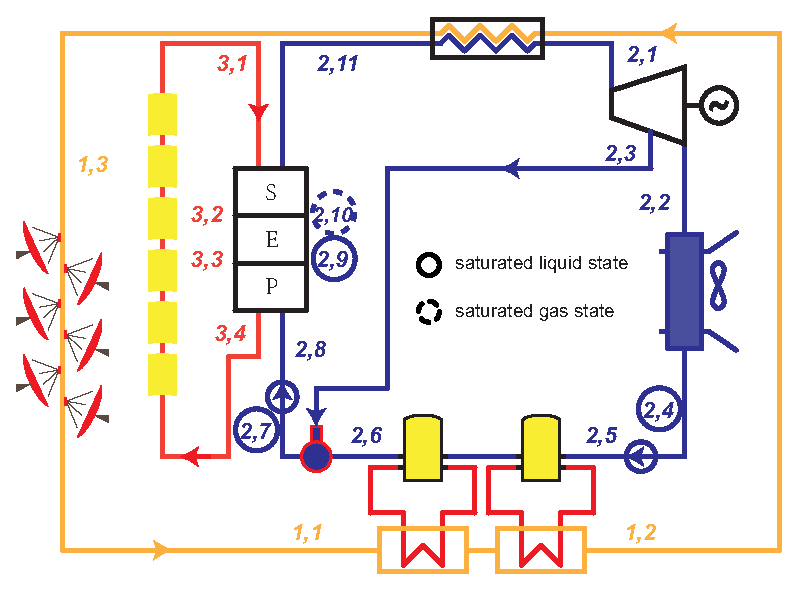
\includegraphics[width = 0.7\columnwidth]{./graphics/cascadeSystem}
	\caption{Sketch of the cascade system}
	\label{fig:System-1}
\end{center}
\end{figure}

%:Should I remove the detailed values?
\noindent \begin{figure}[htbp]
\begin{center}
	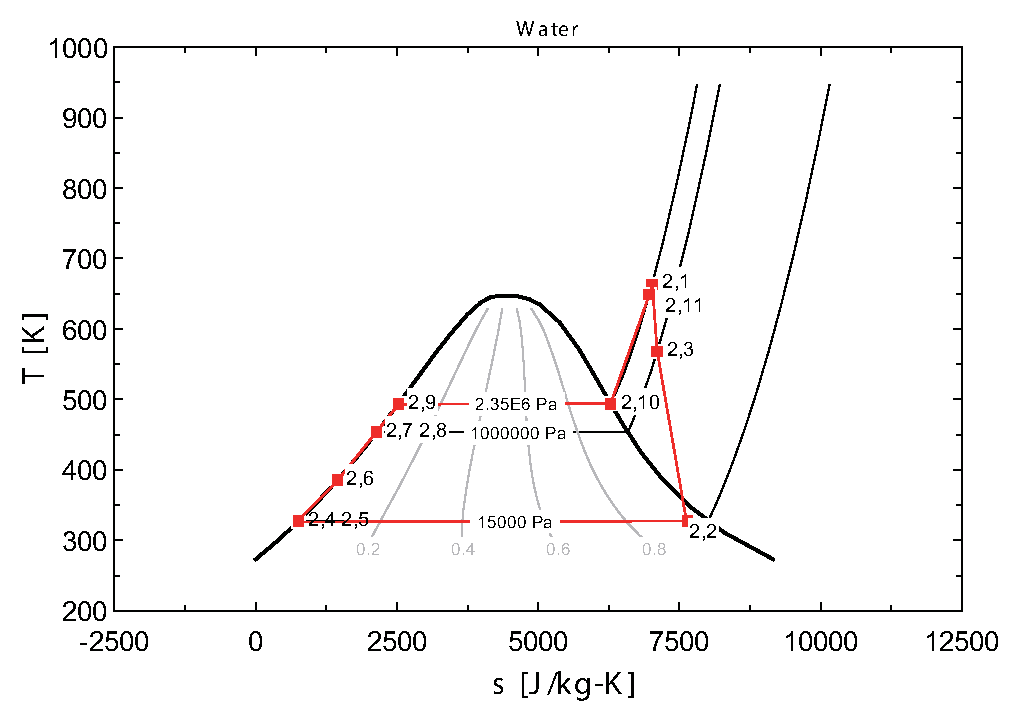
\includegraphics[width = 0.7\columnwidth]{./graphics/T-s_Water}
	\caption{$T-s$ diagram of the water circuit}
	\label{fig:T-s_Water}
\end{center}
\end{figure}

\noindent \begin{figure}[htbp]
\begin{center}
	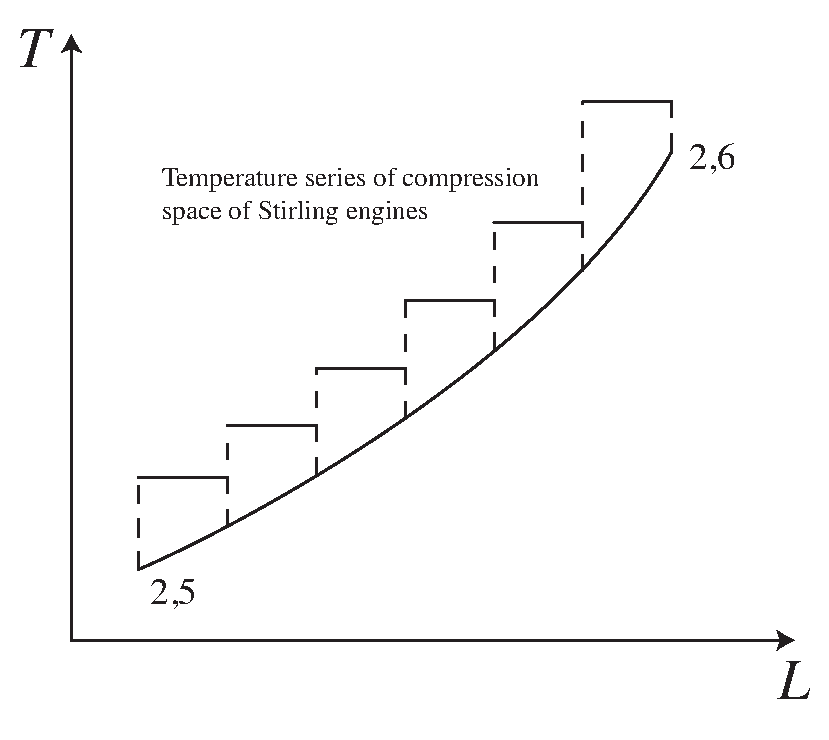
\includegraphics[width = 0.7\columnwidth]{./graphics/HeatTransfer_Water-SEs}
	\caption{Heat transfer diagram of process 2,5-2,6}
	\label{fig:HeatTransfer_Water-SEs}
\end{center}
\end{figure}

To build the cascade system model, several simplifying assumptions are made:

\begin{itemize}
	\item Steady state at nominal load of the system is analyzed
	\item Pressure drop due to flow is negligible
	\item The leak of working fluid in the pipes is neglected
	\item Same isentropic efficiency of steam turbine with different loads and in different stages
	\item Heat loss that occurs from the tube to the atmosphere is not considered
	\item There is no heat loss to the environment for Stirling engines
	\item Simple models are used of some processes and equipments
	\item A symmetrical regenerator behaviour is assumed so that a single effectiveness can be defined as $e=\dfrac{T_R - T_L}{T_H - T_L}$~\cite{Formosa2010,Juhasz2010}
\end{itemize}

%\section{System specification}
Table~\ref{tab:system-data} shows the basic design parameters of the cascade system.

%\begin{table}[htbp]
%	\caption{Parameters of the cascade system}
%	\begin{center}
%	\begin{tabular}{cc}
%		\toprule
%		\multicolumn{2}{c}{Nominal electric power}\\
%		\midrule
%		$P_{generator}$		&	6$\times10^6$ W\\
%		\midrule
%		\multicolumn{2}{c}{Environment}\\
%		\midrule
%		$I_{DNI}$			&	700 W/m$^2$\\
%		$T_{amb}$			&	293 K\\
%		$p_{amb}$			&	1$\times10^5$ Pa\\
%		$v_{wind}$			&	4 m/s\\
%		\midrule
%		\multicolumn{2}{c}{Dish collector}\\
%		\midrule
%		$T_{dish,inlet}$	&	623K\\
%		$T_{dish,outlet}$	&	1073 K\\
%		$p_{dish}$			&	5$\times10^5$ Pa\\ 
%		$A_{dc}$	&	87.7 m$^2$\\
%		\midrule
%		\multicolumn{2}{c}{Trough collector}\\
%		\midrule
%		$\Delta{}T_{oil,water,min}$	&	15 K \\
%		$T_{trough,outlet}$	&	623 K\\
%		$p_{trough}$		&	2$\times10^6$ Pa\\
%		$A_{tc}$	&	545 m$^2$\\
%		\midrule
%		\multicolumn{2}{c}{Stirling engine}\\
%		\midrule
%		$T_{1,afterstirling}$	&	673 K\\
%		$n_{se}$			&	10 s$^{-1}$\\
%		$U_{stirling,1}$	&	30 W/(m$^2\cdot$K)\\
%		$U_{stirling,2}$	&	150 W/(m$^2\cdot$K)\\
%		$A_{stirling,1}$	&	8 m$^2$\\
%		$A_{stirling,2}$	&	8 m$^2$\\
%		$k_{stirling}$		&	1.4\\
%		$\gamma_{stirling}	$	&	3.375\\
%		$n$					&	7.73$\times{}10^{-2}$ mol\\
%		$n_{stirlingEngine}$	&	100\\
%		\midrule
%		\multicolumn{2}{c}{Steam turbine}\\
%		\midrule
%		$T_s$				&	340$^\circ$C\\
%		$p_s$				&	2.35$\times10^6$ Pa\\
%		$p_c$				&	1.5$\times10^4$ Pa\\
%		$T_{s,d}$			&	390$^\circ$C\\
%		$p_{c,p}$			&	1$\times10^6$ Pa\\
%		\midrule
%		\multicolumn{2}{c}{Deaerator}\\
%		\midrule
%		$p_{deaerator}$ & 1$\times10^6$ Pa\\
%		\bottomrule
%	\end{tabular}
%	\end{center}
%	\label{tab:system-data}
%\end{table}
\begin{table}[htbp]
	\caption{Basic design parameters of the cascade system}
	\begin{center}
	\begin{tabular}{cc}
		\toprule
		Parameters			&	Value\\
		\midrule
		$I_r$			&	700 W/m$^2$\\
		$T_{amb}$			&	293 K\\
		$p_{amb}$			&	1$\times10^5$ Pa\\
		$v_{wind}$			&	4 m/s\\
		$P_{generator}$		&	6$\times10^6$ W\\
		$T_{dish,inlet}$	&	623K\\
		$T_{dish,outlet}$	&	1073 K\\
		$p_{dish}$			&	5$\times10^5$ Pa\\
		$\Delta{}T_{oil,water,min}$	&	15 K \\
		$T_{trough,outlet}$	&	623 K\\
		$p_{trough}$		&	2$\times10^6$ Pa\\
		$T_{1,afterstirling}$	&	673 K\\
		$n_{stirlingEngine}$	&	100\\
		$T_s$				&	340$^\circ$C\\
		$p_s$				&	2.35$\times10^6$ Pa\\
		$p_c$				&	1.5$\times10^4$ Pa\\
		$T_{s,d}$			&	390$^\circ$C\\
%		$p_{c,p}$			&	1$\times10^6$ Pa\\
		$p_{deaerator}$ 	& 	1$\times10^6$ Pa\\
		\bottomrule
	\end{tabular}
	\end{center}
	\label{tab:system-data}
\end{table}
\nomenclature{$P_{generator}$}{Power of generator, W}
\nomenclature{$I_r$}{Direct Normal Irradiance, W/m$^2$}
\nomenclature{$T_{amb}$}{Ambient temperature, K}
\nomenclature{$p_{amb}$}{Ambient pressure, Pa}
\nomenclature{$v_{wind}$}{Ambient wind speed, m/s}
\nomenclature{$T_{dish,inlet}$}{Dish inlet temperature, K}
\nomenclature{$T_{dish,outlet}$}{Dish outlet temperature}
\nomenclature{$p_{dish}$}{Air pressure in dish, Pa}
\nomenclature[S]{$dc$}{Dish collector}
\nomenclature[G]{$\Delta{}T_{oil,water,min}$}{Minimum temperature difference between oil and water in the oil-to-water heat exchanger, K}
\nomenclature{$T_{trough,outlet}$}{Trough outlet temperature}
\nomenclature{$p_{trough}$}{Air pressure in trough, Pa}
\nomenclature[S]{$tc$}{Trough collector}
\nomenclature{$T_{1,afterstirling}$}{Air temperature after heating Stirling engine}
\nomenclature{$n_{se}$}{Speed of Stirling engine, s$^{-1}$}
\nomenclature{$U_{stirling,1}$}{Overall heat transfer coefficient of Stirling engine at air side, W/(m$^2\cdot$K)}
\nomenclature{$U_{stirling,2}$}{Overall heat transfer coefficient of Stirling engine at water side, W/(m$^2\cdot$K)}
\nomenclature{$T_s$}{Main steam temperature of turbine}
\nomenclature{$p_s$}{Main steam pressure of turbine, Pa}
\nomenclature{$p_c$}{Exhaust pressure of turbine, Pa}
\nomenclature{$T_{s,d}$}{Designed mean steam temperature of turbine}
\nomenclature{$p_{deaerator}$}{Pressure of deaerator, Pa}
\nomenclature[S]{1}{First fluid, Air}
\nomenclature[S]{2}{Second fluid, Water}

\section{System model}
An EES\nomenclature[C]{EES}{Engineering Equation Solver} model was built to investigate the characteristics of the cascade system. The cascade system is built in several blocks. These blocks are made of circuits with efficiency calculations. Three circuits, air circuit, water circuit and oil circuit, are built with some specific state parameters in some key components. Energy-based models of these key components are created on the basis of their thermodynamic behavior, heat transfer and the second law.

The following parts introduce models of some key components.

\subsection{Dish collector}
The most complicate part of the dish collector is the dish receiver. In our cascade system, the structure of the dish receiver is as shown in Figure~\ref{fig:dishReceiver}. This section mainly describes dish receiver.

\noindent \begin{figure}[htbp]
\begin{center}
	\includegraphics[width = 0.7\columnwidth]{graphics/dishReceiver1}
	\caption{Structure of the dish receiver}
	\label{fig:dishReceiver}
\end{center}
\end{figure}

Fraser, in his dissertation~\cite{Fraser2008}, built a performance prediction model of Stirling dish system with detailed description. The model is also used in the software SAM\nomenclature[C]{SAM}{System Advisor Model}, which provides performance and financial models for facilitate decision in the renewable energy industry. The dish collector model in the dissertation considers various heat losses, which is a good reference for the dish receiver model of the cascade system. 

A dish collector product of SES\nomenclature[C]{SES}{Stirling Energy System} used in Fraser's dissertation, which is also used in this system, and its parameters are listed in Table~\ref{tab:dc}~\cite{Fraser2008}. 

\begin{table}[htbp]
	\caption{Parameters of the dish collector}
	\begin{center}
	\begin{tabular}{cc}
		\toprule
		Parameters	&	Value\\
		\midrule
		$d_{cav}$	&	0.46 m\\
		$\delta_{insu}$	&	0.075 m\\
		$dep_{cav}$	&	0.23 m\\
		$d_{ap}$	&	0.184 m\\
		$\lambda_{insu}$	&	0.06 W/(m$\cdot$K)\\
		$\epsilon_{insu}$	&	0.6\\
		$\alpha_{cav}$	&	0.87\\
		$\delta_a$	&	0.005 m\\
		$d_{i,air}$	&	0.07 m\\
		$A_{dc}$	&	87.7 m$^2$\\
		$\theta_{dish}$	&	45$^\circ$\\
		$\gamma$	&	0.97\\
		$\eta_{shading}$	&	0.95\\
		$\rho$	&	0.91\\
		\bottomrule
	\end{tabular}
	\end{center}
	\label{tab:dc}
\end{table}
\nomenclature[G]{$\delta_{insu}$}{Thickness of receiver insulating layer, m}
\nomenclature{$dep$}{Depth, m}
\nomenclature{$d$}{Diameter, m}
\nomenclature[G]{$\lambda_{insu}$}{Thermal conductivity of receiver insulating layer, W/(m$\cdot$K)}
\nomenclature[G]{$\epsilon_{insu}$}{Emissivity of reciver insulating layer}
\nomenclature[G]{$\delta_{a}$}{Thickness of air tube in volumetric receiver, m}
\nomenclature{$d_{i,air}$}{Inner diameter of air tube, m}
\nomenclature[G]{$\theta_{dish}$}{Dish aperture angle (0$^{\circ}$ is horizental, 90$^{\circ}$ is vertically down)}
\nomenclature[G]{$\gamma$}{Intercept factor}
\nomenclature[G]{$\eta_{shading}$}{Shading factor}
\nomenclature[G]{$\rho$}{Reflectivity}
\nomenclature{$A_{stirling,1}$}{Heat transfer area of Stirling engine at air side, m$^2$}
\nomenclature{$A_{stirling,2}$}{Heat transfer area of Stirling engine at water side, m$^2$}
\nomenclature{$k_{stirling}$}{Specific heat ratio of the working gas in Stirling engine}
\nomenclature[G]{$\gamma_{stirling}$}{Compression ratio of Stirling engine}
\nomenclature{$n_g$}{Amount of working gas in each Stirling engine, mol}
\nomenclature{$n_{stirlingEngine}$}{Number of Stirling engines in the Stirling engine array}

The dish receiver model concerns the losses include: collector losses due to mirror reflectivity, receiver intercept losses, losses due to shading, and thermal losses. Thermal losses take the largest portion of all those losses, which are due to conduction, convection and radiation. Figure~\ref{fig:thermal-lose} shows the heat network of dish receiver, which concerns the losses:
\begin{itemize}
	\item Radiation losses reflected off of the receiver cavity surfaces and out of the receiver through the aperture. ($q_{rad,reflect}$)
	\item Conductive losses through the receiver insulating layer. ($q_{cond,tot}$)
	\item Free convection from the cavity in the absence of wind. ($q_{conv,free}$)
	\item Forced convection in the presence of wind. ($q_{conv,forced}$)
	\item Emission losses due to thermal radiation emitted from the receiver aperture. ($q_{rad,emit}$)
\end{itemize}

\noindent \begin{figure}[htbp]
\begin{center}
	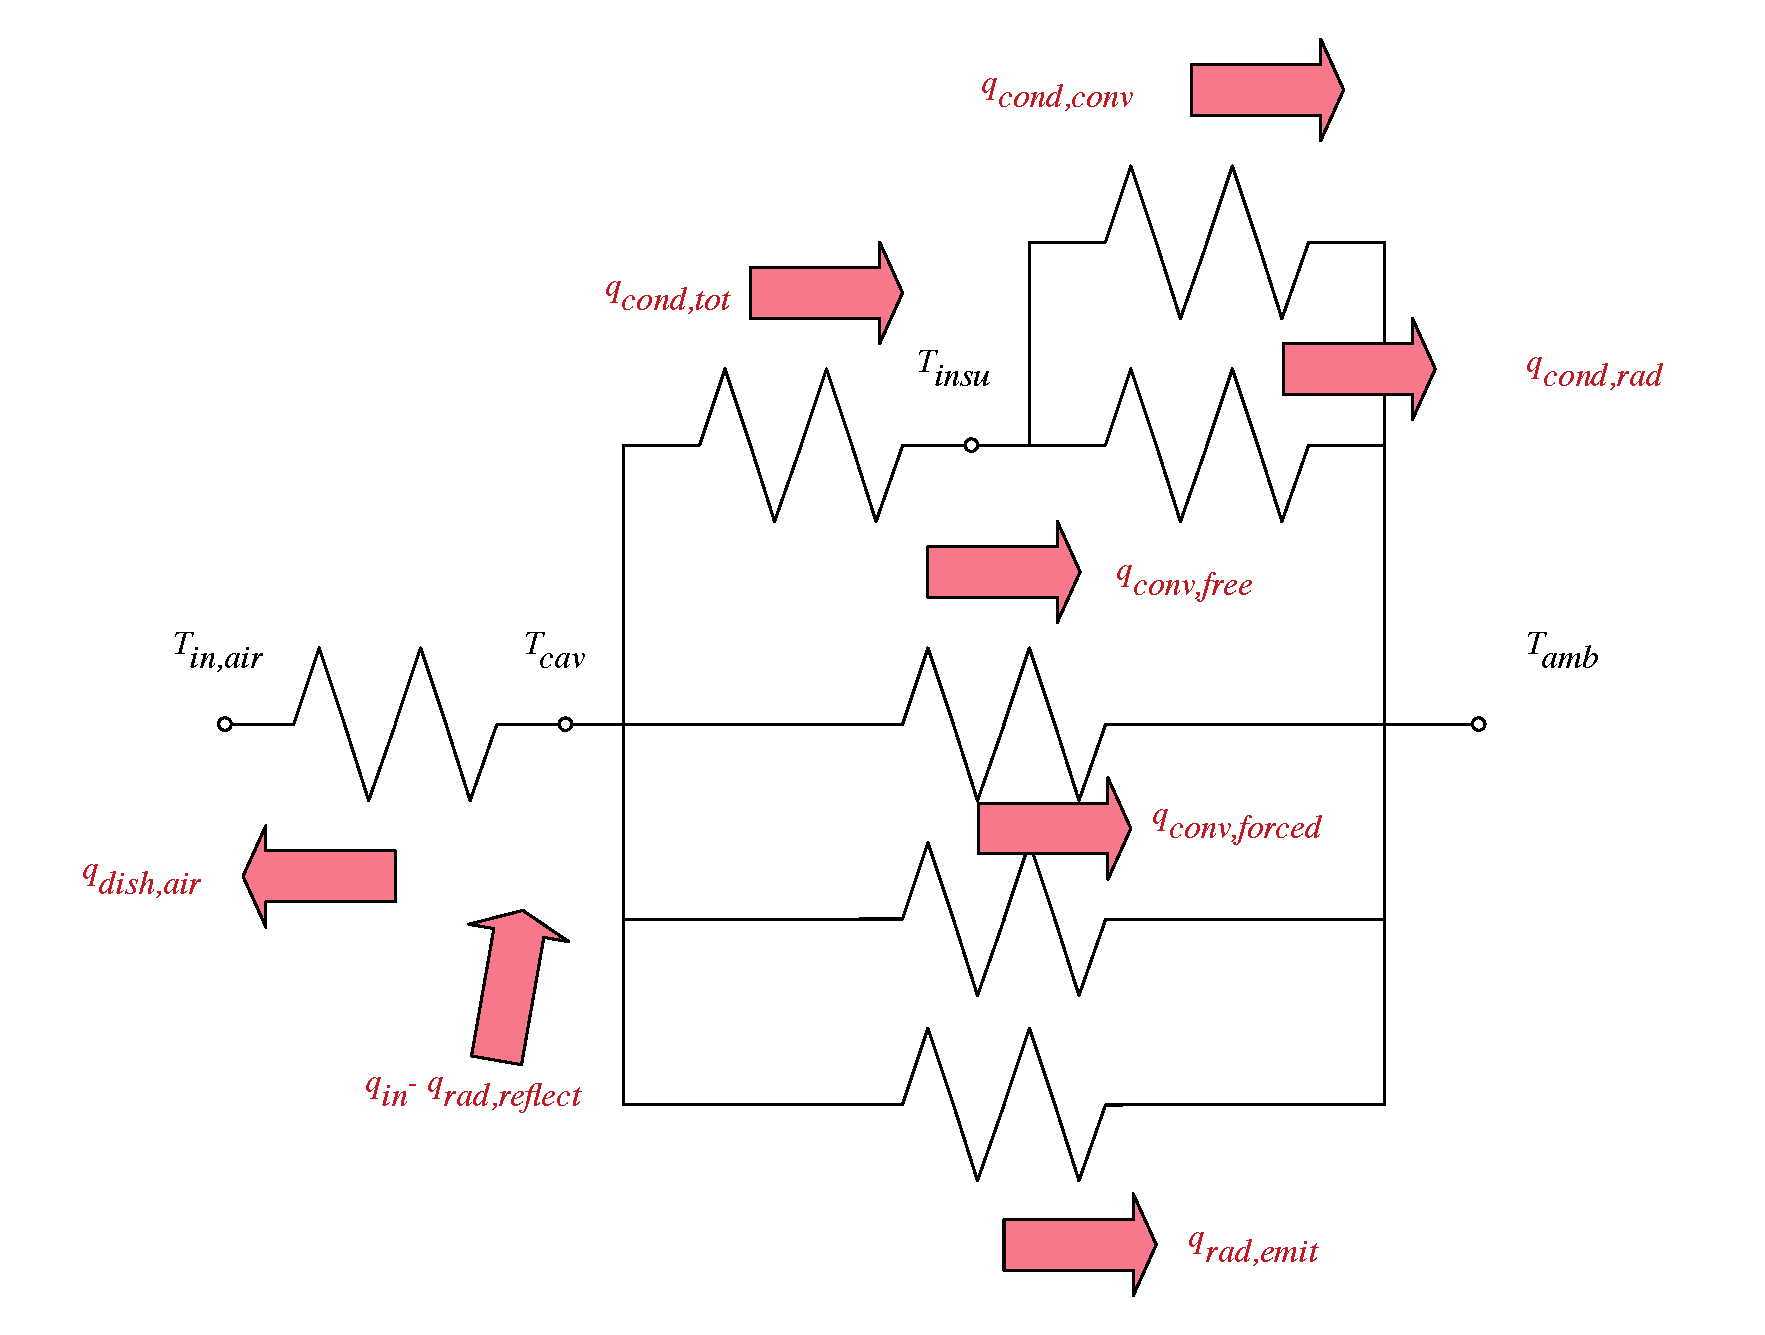
\includegraphics[width = 0.7\columnwidth]{./graphics/thermalLosses}
	\caption{Heat network of dish receiver}
	\label{fig:thermal-lose}
\end{center}
\end{figure}

$q_{dish,air}$ can be written as
\begin{equation*}
	q_{dish,air}=h_{dish,air}A_{dish,air}\Delta{}T_{ln,Drec,air}
\end{equation*}
\nomenclature{$A_{dish,air}$}{Heat transfer area of dish receiver between tube and air, m$^2$}

where

\begin{equation*}
	h_{dish,air}=Nu_{tube}\lambda_{dish,air}/d_{i,air}
\end{equation*}
\nomenclature{$Nu$}{Nusselt number}

\begin{equation*}
	Nu_{tube}=c_rNu_{tube}^{'}
\end{equation*}
\nomenclature{$c_r$}{Heat transfer correction factor of coiled tube of volumetric receiver}

For helical spiral pipe, multiplier $c_r$ based on curvature ratio can be written as~\cite{Pablo2008}

\begin{equation*}
	c_{r}=1+3.5\frac{d_{i,air}}{d_{cav}-d_{i,air}-2\delta_{a}}
\end{equation*}

$Nu_{tube}^{'}$ is the Nusselt number of straight circular tube, which can be obtained by~\cite{Serth2007}

\begin{equation*}
	Nu_{tube}^{'}= 0.027Re_{tube}^{0.8}Pr_{tube}^{1/3}(\mu_{tube}/\mu_{tube,w})^{0.14}
\end{equation*}
\nomenclature{$Pr$}{Prandtl number}
\nomenclature{$Re$}{Reynolds number}
\nomenclature[G]{$\mu$}{Viscosity, kg/(m$\cdot$s)}
\nomenclature[S]{$w$}{Tube wall}

\begin{equation*}
	c_{r}=1+3.5\frac{d_{i,air}}{d_{cav}-d_{i,air}-2\delta_{a}}
\end{equation*}

and $\Delta{}T_{ln,Drec,air}$ can be written as

\begin{equation*}
	\Delta{}T_{ln,Drec,air}=\frac{(T_{cav}-T_{dish,inlet})-(T_{cav}-T_{dish,outlet})}{\ln\dfrac{T_{cav}-T_{dish,inlet}}{T_{cav}-T_{dish,outlet}}}
\end{equation*}

To get $q_{dish,air}$, $T_{cav}$ is required. As shown in Figure~\ref{fig:thermal-lose}, we need to solve the heat network.

\begin{equation}
\begin{aligned}
	q_{in} = q_{rad,reflect}+q_{dish,air}+q_{cond,tot}+q_{conv,tot}+
	\\q_{rad,emit}\label{eq:q_in sum}
\end{aligned}
\end{equation}
\nomenclature{$q_{in}$}{Solar energy launched into dish receiver aperture, W}
\nomenclature{$q_{rad,reflect}$}{Reflected radiation by volumetric receiver, W}
\nomenclature{$q_{dish,air}$}{Energy absorbed by air in the dish collector}
\nomenclature{$q_{cond,tot}$}{Total conduction loss}
\nomenclature{$q_{conv,tot}$}{Total convection loss}
\nomenclature{$q_{rad,emit}$}{Radiation emitted by dish receiver}


$q_{in}$ and $\eta_{dc}$ can be obtained by
\nomenclature[G]{$\eta$}{Thermal efficiency}

\begin{equation}
	q_{in}=I_r\cdot A_{dc}\gamma\eta_{shading}\rho
	\label{eq:q_in}
\end{equation}

\begin{equation}
	\eta_{dc}=q_{dish,air}/\left(I_r\cdot A_{dc}\right)
	\label{eq:eta_dc}
\end{equation}

Other losses are presented in following sections.

\subsubsection{Reflected loss of dish receiver}
To determine the reflected loss of the cavity surfaces of the dish receiver $q_{rad,reflect}$, the effective absorptance of the cavity receiver $\alpha_{eff}$\nomenclature[S]{$eff$}{Effective parameter of the dish receiver cavity} is required to determine the fraction of energy reflected out of the receiver. The effective absorptance of a cavity receiver without a receiver aperture cover is given by Equation~(\ref{eq:alpha_eff}) where $\alpha_{cav}$ is the cavity surface absrptance, $A_a$ is the cavity aperture area, and $A_{cav}$ is the total inner surface area of the cavity~\cite{Duffie2013}. Sandra National Laboratories gave an estimate value of the absorptance of the cavity surface $\alpha_{cav}$ of an existing Stirling dish receiver to be 0.87~\cite{Hogan1994}. To achieve higher effective absorptance, a smaller ratio of the two surface area should be used. But the ratio is constrained by the concentration ratio of the receiver.

\begin{equation}
	\alpha_{eff}=\dfrac{\alpha_{cav}}{\alpha_{cav}+\left(1-\alpha_{cav}\right)\left(A_{ap}/A_{cav}\right)}
	\label{eq:alpha_eff}
\end{equation}
\nomenclature[G]{$\alpha$}{Absorptance}
\nomenclature[S]{$ap$}{Aperture of the dish receiver}
\nomenclature[S]{$cav$}{Cavity of the dish receiver}

\begin{equation*}
	q_{rad,reflect}=q_{in}(1-\alpha_{eff})
\end{equation*}

\subsubsection{Conduction loss of dish receiver}
Conduction loss of dish receiver $q_{cond,tot}$ equals to the different two parts: convection loss from the insulating layer to the atmosphere $q_{cond,conv}$ and radiation loss from the insulating layer to the atmosphere $q_{cond,rad}$. Both of the two parts are related to the temperature of insulating layer $T_{insu}$.
\nomenclature{$T_{insu}$}{Temperature of insulating outside layer, K}

\begin{equation*}
	q_{cond,tot}=\dfrac{T_{cav}-T_{insu}}{\ln\dfrac{d_{cav}+2\delta_{insu}}{d_{cav}}/(2\pi\lambda_{insu}dep_{cav})}
\end{equation*}
\begin{equation*}
\begin{split}
	q_{cond,conv}=h_{insu}A_{insu}(T_{insu}-T_{amb})
	\\=\dfrac{k_{insu}Nu_{insu}A_{insu}(T_{insu}-T_{amb})}{d_{cav}+2\delta_{insu}}
\end{split}
\end{equation*}
\nomenclature{$k_{insu}$}{Thermal conductivity of air at the temperature of outside insulating layer, W/(m$\cdot$K)}

where $Nu_{insu}$ can be obtained by the correlation for flow over a circular cylinder.~\cite{Churchill1977} 

\begin{equation*}
	q_{cond,rad}=\epsilon_{insu}A_{insu}\sigma(T_{insu}^4 - T_{amb}^4)	
\end{equation*}
And 
\begin{equation*}
	q_{cond,tot}=q_{cond,conv}+q_{cond,rad}	
\end{equation*}

\subsubsection{Convection loss of dish receiver}
Ma~\cite{Ma1993} conducted tests to determine the free convection losses from the receiver for alternative setups, and the data were consistent with Stine and McDonald's free convection correlation. It is assumed that forced convection is independent of free convection in the receiver, so the total convection losses can be represented as the sum of the free and forced convection losses as shown in Figure~\ref{fig:thermal-lose}.

\begin{equation*}
	q_{con,tot} = (h_{free} + h_{forced})A_{cav}(T_{cav}-T_{amb})
\end{equation*}


where $h_{free}=k_{film}Nu_{free}/\overline{d_{cav}}$, $\overline{d_{cav}}=d_{cav}-2d_i-4 \delta_a$.
\nomenclature{$\overline{d_{cav}}$}{Effective diameter of the cavity, m}
\nomenclature{$d_i$}{Inner diameter of trough receiver, m}$d_{i}=0.066\,$m

Wu~\cite{Wu2010} present a comprehensive review and systematic summarization of convection heat loss from cavity receiver in parabolic dish solar thermal power system. And we choose the correlation presented by Leibfried~\cite{Leibfried1995}. This correlation gives an extended model of Koenig~\cite{Koenig1981} and Stine~\cite{Stine1994} with better results.

For forced convection loss, side-on wind convection loss model given by Ma~\cite{Ma1993}, which is independent of the aperture orientation, is used

\begin{equation*}
	h_{forced}=0.1967v_{wind}^{1.849}
\end{equation*}

\subsection{Trough collector}

LS-3 is used as the trough collector, its sketch is shown in Figure~\ref{fig:tc}, its parameters are listed in Table~\ref{tab:tc}.

\noindent \begin{figure}[htbp]
\begin{center}
	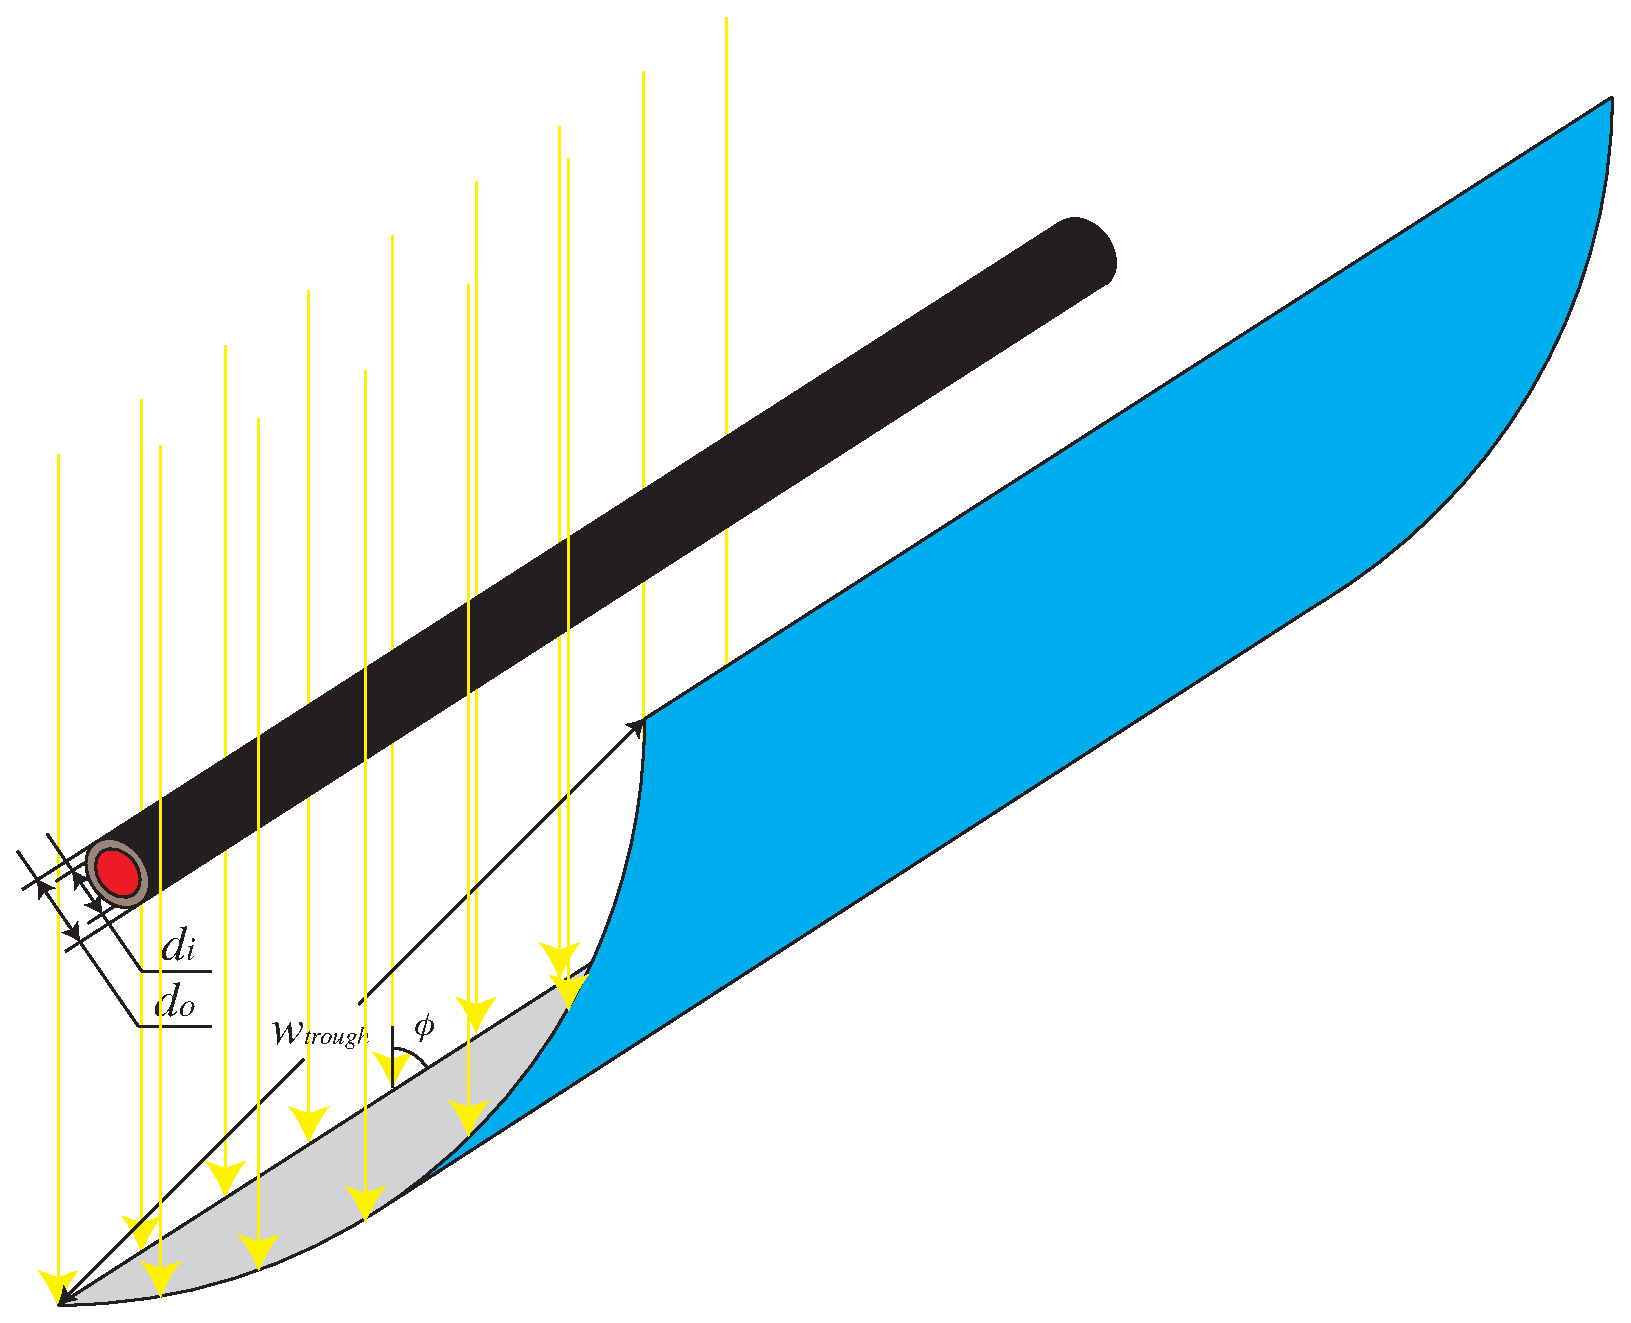
\includegraphics[width = 0.7\columnwidth]{./graphics/TroughCollector}
	\caption{Sketch of trough collector}
	\label{fig:tc}
\end{center}
\end{figure}

\begin{table}[htbp]
	\caption{Parameters of the trough receiver}
	\begin{center}
	\begin{tabular}{cc}
		\toprule
		Parameters	&	Value\\
		\midrule
		$A_{tc}$	&	545 m$^2$\\
		$w_{trough}$&	5.76 m\\
		$d_i$		&	0.066 m\\
		$d_o$	&	0.07 m\\
		$\rho$		&	0.94\\
		$\gamma$	&	0.93\\
		$\tau$		&	0.95\\
		$\alpha_{abs}$	&	0.96\\
		$F_e$		&	0.97\\
		$\phi$	&	70$^\circ$\\
		\bottomrule
	\end{tabular}
	\end{center}
	\label{tab:tc}
\end{table}
\nomenclature{$d_o$}{Outer diameter of trough receiver, m}
\nomenclature{$F_e$}{Soiling factor of the trough collector}
\nomenclature{$w_{trough}$}{Width of trough collector, m}
\nomenclature[G]{$\phi$}{Incidence angle}

\begin{equation*}
	q^{''}=I_rw_{trough}\eta_{opt,0}K(\phi)F_{e}/P
\end{equation*}

where $P=\pi{}d$, $K(\phi)$ is the incidence angle modifier, $\eta_{opt,0}$
is peak optical efficiency (optical efficiency with an incidence angle of 0).
\nomenclature{$K$}{Incidence angle modifier of trough collector}
\nomenclature[G]{$\eta_{opt,0}$}{Optical efficiency with an incidence angle of 0}

Assume overall heat transfer coefficient $U(T_{abs})$ is uniform for whole length, so that we can use the heat transfer correlation in Appendix~\ref{sec:CTCHTHT}.
\nomenclature{$U$}{Overall heat transfer coefficient, W/(m$^2\cdot$K)}
\nomenclature{$q^{''}$}{Heat flux, W/m$^2$}

\begin{equation}
	\frac{T_{o}-T_{amb}-\dfrac{q^{''}}{U(T_{abs})}}{T_{i}-T_{amb}-\dfrac{q^{''}}{U(T_{abs})}}=\exp(-\frac{U(T_{abs})PL}{q_{m}c_{p}})\label{eq:CTCHF}
\end{equation}

Since the $Nu$ in the pipe is very large (about $1\times10^4$), small temperature difference exists between the absorber and oil. So $(T_{i}+T_{o})/2$ can be used as the average value of $T_{abs}$, and $U(T_{abs})$ can be obtained by the a second-order polynomial function given by Romero\cite{Romero2007}. Then using Equation (\ref{eq:CTCHF}), we can get the length $L$ required to get the required number of trough collectors in a row.

The efficiency of the trough collector

\begin{equation*}
	\eta_{trough}=\frac{q_m(h_{out}-h_{in})}{I_rw_{trough}L}
\end{equation*}

\subsection{Stirling engine array}

Stirling engine array is used in the cascade system, Figure~\ref{fig:Layout of Stirling engines} shows the layout of the Stirling engine array. Each Stirling engine in the Stirling engine array has the identical parameters: $U_{stirling,1}=30\,$W/m$^2\cdot$K, $U_{stirling,2}=150\,$W/m$^2\cdot$K, $A_{stirling,1}=6\,$m$^2$, $A_{stirling,2}=6\,$m$^2$, $k_{stirling}=1.4$, $\gamma_{stirling}=3.375$, $n_g=7.84\times{}10^{-2}\,$mol, $n_{se}=10\,$s$^{-1}$.

\noindent \begin{figure}[htbp]
\begin{center}
	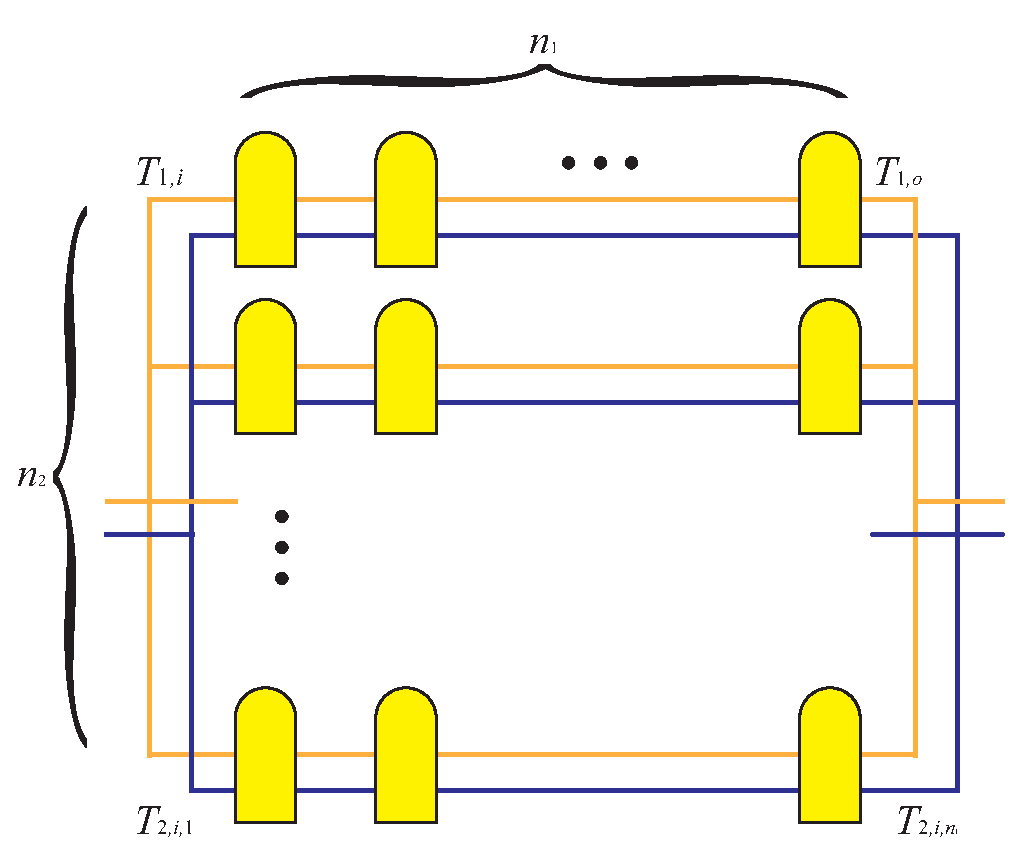
\includegraphics[width = 0.7\columnwidth]{./graphics/StirlingEngineArray}
	\caption{Layout of Stirling engines}
	\label{fig:Layout of Stirling engines}
\end{center}
\end{figure}

Depending on the flow directions of heating and cooling flows, there are two flow types: parallel flow and counter flow. Figure~\ref{fig:ParallelFlow} and Figure~\ref{fig:CounterFlow} show the heat transfer diagrams of the two flow types.
%: \nomenclature{$n_1$}{Number of columns of the Stirling engine array} $n_1$ is chosen to be 10 and can be optimized later. 

\noindent \begin{figure}[htbp]
\begin{center}
	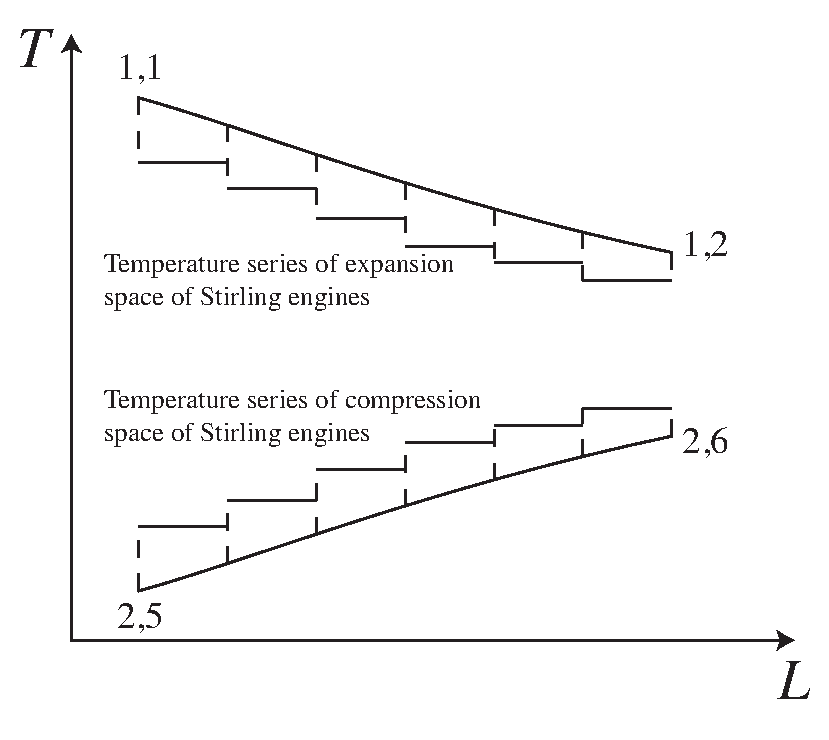
\includegraphics[width = 0.7\columnwidth]{./graphics/HeatTransfer_Parallel}
	\caption{Heat transfer diagram of parallel flow}
	\label{fig:ParallelFlow}
\end{center}
\end{figure}

\noindent \begin{figure}[htbp]
\begin{center}
	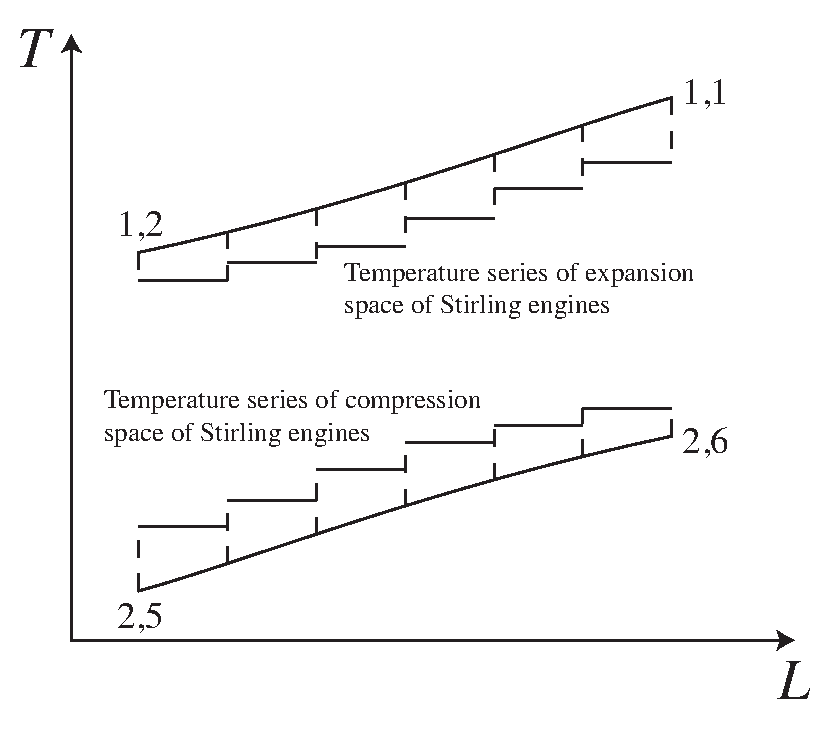
\includegraphics[width = 0.7\columnwidth]{./graphics/HeatTransfer_Counter}
	\caption{Heat transfer diagram of Counter flow}
	\label{fig:CounterFlow}
\end{center}
\end{figure}

In Figure~\ref{fig:Layout of Stirling engines}, $T_{1,i,1}=T_{1,i},q_{m,1,r}=q_{m,1}/n_{2}$. For $x$ from $1$ to $n_1-1$, where $x$ is the column number of Stirling engines, $T_{1,i,x+1}=T_{1,o,x},T_{2,i,x+1}=T_{2,o,x}$.
\nomenclature{$n_1$}{Number of columns of the Stirling engine array}
\nomenclature{$q_{m,1}$}{Total mass flow rate of air, kg/s}

Assume that the positive flow direction is to the right, for parallel flow,
\nomenclature{$n_2$}{Number of rows of the Stirling engine array}
\nomenclature{$q_{m,1,r}$}{Mass flow rate of air in each row of Stirling engine array, kg/s}

\begin{equation*}
	T_{2,i,1}=T_{2,i}\label{eq:T_2_i_1}
\end{equation*}
\begin{equation*}
	q_{m,2,r}=q_{m,2}/n_{2}
\end{equation*}
\nomenclature{$q_{m,2,r}$}{Mass flow rate of water in each row of Stirling engine array, kg/s}
\nomenclature{$q_{m,2}$}{Total mass flow rate of water, kg/s}

for counter flow,

\begin{equation*}
	T_{2,o,n_1}=T_{2,i}\label{eq:T_2_o_n1}
\end{equation*}
\begin{equation*}
	q_{m,2,r}=-q_{m,2}/n_{2}
\end{equation*}

For a Stirling engine in column $x$\nomenclature[S]{$x$}{Stirling engine in column $x$}, $x$ from $1$ to $n_1$, according to Appendix~\ref{sec:Stirling-engine-model},

\begin{equation*}
	T_{H,x}=T_{1,i,x}-\dfrac{T_{1,i,x}-T_{1,o,x}}{1-\exp(-\dfrac{U_{stirling,1}A_{stirling,1}}{q_{m,1,r}c_{p,1,x}})}\label{eq:T_H_x}
\end{equation*}


\begin{equation*}
	T_{L,x}=T_{2,i,x}-\dfrac{T_{2,i,x}-T_{2,o,x}}{1-\exp(-\dfrac{U_{stirling,2}A_{stirling,2}}{q_{m,2,r}c_{p,2,x}})}\label{eq:T_L_x}
\end{equation*}

Assuming a linear temperature profile across the regenerator, the mean effective temperature $T_{R,x}=\dfrac{T_{H,x}-T_{L,x}}{\ln(T_{H,x}/T_{L,x})}$~\cite{Der2007,Cavazzuti2012}, and the symmetrical regenerator behaviour assumption $e_{x}=\dfrac{T_{R,x}-T_{L,x}}{T_{H,x}-T_{L,x}}$~\cite{Formosa2010,Juhasz2010}, then the efficiency of each Stirling engine in column $x$ can be written as~\cite{Stine1985,Goswami2015}

\begin{equation*}
	\eta_{stirling,x}=\dfrac{T_{H,x}-T_{L,x}}{T_{H,x}+\dfrac{1-e_{x}}{k-1}\cdot\dfrac{T_{H,x}-T_{L,x}}{\ln\gamma_{stirling}}}\label{eq:eta_striling_x}
\end{equation*}

For energy balance,

\begin{equation*}
	q_{m,1,r}(h_{1,i,x}-h_{1,o,x})(1-\eta_{stirling,x})=q_{m,2,r}(h_{2,o,x}-h_{2,i,x})
\end{equation*}

And in each Stirling cycle, the heat absorbed by the working gas is 
\begin{equation*}
\begin{split}
	n_gR\left(T_{H,x}\ln\gamma_{stirling}+\dfrac{1-e_{x}}{k-1}\left(T_{H,x}-T_{L,x}\right)\right)=\\q_{m,1,r}(h_{1,i,x}-h_{1,o,x})/n_{se}
\end{split}
\end{equation*}

By solving above equations, efficiency of the Stirling engine array $\eta_{stirling}$ can be obtained by

\begin{equation*}
	\eta_{stirling}=1-\dfrac{q_{m,2}(h_{2,o,n_1}-h_{2,i,1})}{q_{m,1}(h_{1,i,1}-h_{1,o,n_1})}\label{eq:eta_stirling-1}
\end{equation*}


and power of each Stirling engine in column $x$
\begin{equation*}
	P_{stirlingEngine,x}=q_{m,1,r}(h_{1,i,x}-h_{1,o,x})\eta_{stirling,x}
\end{equation*}


and power of the Stirling engine array
\begin{equation*}
	P_{stirling}=\eta_{stirling}q_{m,1}(h_{1,i,1}-h_{1,o,n_1})
\end{equation*}

\subsection{Steam turbine}

A steam turbine product, N-6 2.35, of Qingdao Jieneng Power Station Engineering Co., Ltd is used for calculation. Its isentropic efficiency $\eta_{i,turbine}$ can be obtained by the given design parameters.
\nomenclature[S]{$i$}{Isentropic}

Using basic design parameters in Table~\ref{tab:system-data}, parameters of state 2,2 and 2,3 in Figure~\ref{fig:System-1} of the steam turbine can be obtained by the following equations.

\begin{equation*}
	\eta_{i,turbine}=\frac{h_{2,1}-h_{2,2}}{h_{2,1}-h_{i,2,2}}
\end{equation*}

\begin{equation*}
	\eta_{i,turbine}=\frac{h_{2,1}-h_{2,3}}{h_{2,1}-h_{i,2,3}}
\end{equation*}

The output power of steam turbine

\begin{equation*}
	P_{turbine}=\left(1-y\right)q_{m,2}\left(h_{2,1}-h_{2,2}\right)+yq_{m,2}\left(h_{2,1}-h_{2,3}\right)
\end{equation*}
\nomenclature{$y$}{Extraction rate of steam turbine}

The sum power of pumps

\begin{equation*}
	P_{pump}=\left(1-y\right)q_{m,2}\left(h_{2,5}-h_{2,4}\right)+q_{m,2}\left(h_{2,8}-h_{2,7}\right)
\end{equation*}

Heat injected in the water circuit

\begin{equation*}
	Q_2=\left(1-y\right)q_{m,2}\left(h_{2,6}-h_{2,5}\right)+q_{m,2}\left(h_{2,1}-h_{2,8}\right)
\end{equation*}

The efficiency of Rankine cycle can be expressed as

\begin{equation*}
	\eta_{rankine}=(P_{turbine}-P_{pump}/\eta_{generator})/Q_{2}
\end{equation*}

%\subsubsection{Condensor}
%
%\subsubsection{deaerator}

\section{Separate system models}

\noindent \begin{figure}[htbp]
\begin{center}
	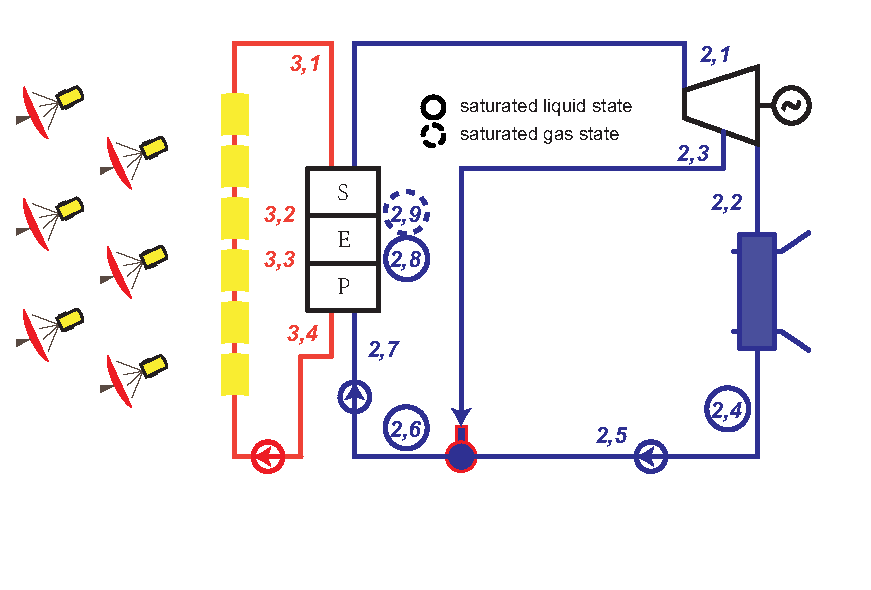
\includegraphics[width = 0.7\columnwidth]{./graphics/separateSystem}
	\caption{Sketch of the separate systems}
	\label{fig:System-2}
\end{center}
\end{figure}

Figure~\ref{fig:System-2} shows the sketch of the separate systems. These two separate systems were built for comparison. They use the same dish collectors and trough collectors with the same thermal efficiencies.

\subsection{Separate trough system}

Steam turbine has the same main parameters and same isentropic efficiency with that of the cascade system. Pressure of deaerator are the same of the cascade system. So parameters of state 2,2 and 2,3 in Figure~\ref{fig:System-2} of the steam turbine can be obtained by the following equations.

\begin{equation*}
	\eta_{i,turbine}=\frac{h_{2,1,s}-h_{2,2,s}}{h_{2,1,s}-h_{i,2,2,s}}
\end{equation*}
\nomenclature[S]{$s$}{Separate systems}

\begin{equation*}
	\eta_{i,turbine}=\frac{h_{2,1,s}-h_{2,3,s}}{h_{2,1,s}-h_{i,2,3,s}}
\end{equation*}

The output power of steam turbine

\begin{equation*}
	P_{turbine,s}=\left(1-y_{s}\right)q_{m,2,s}\left(h_{2,1,s}-h_{2,2,s}\right)+y_{s}q_{m,2,s}\left(h_{2,1,s}-h_{2,3,s}\right)
\end{equation*}

The output power of generator

\begin{equation*}
	P_{generator,s}=P_{turbine,s}\eta_{generator}
\end{equation*}

The sum power of pumps

\begin{equation*}
	P_{pump,s}=\left(1-y_{s}\right)q_{m,2,s}\left(h_{2,5,s}-h_{2,4,s}\right)+q_{m,2,s}\left(h_{2,7,s}-h_{2,6,s}\right)
\end{equation*}

Heat injected in the water circuit

\begin{equation*}
	Q_{2,s}=q_{m,2,s}\left(h_{2,1,s}-h_{2,7,s}\right)
\end{equation*}

The generator efficiency is the same of that in the cascade system, and the efficiency of Rankine cycle can be expressed as

\begin{equation*}
	\eta_{rankine,s}=(P_{turbine,s}-P_{pump,s}/\eta_{generator})/Q_{2,s}
\end{equation*}

\subsection{Separate dish system}

In the separate dish system, Stirling engines with the same number of dish collectors are directly put on the focuses of the dish collectors. Water is used for cooling the Stirling engines.

$T_{H,s}$ is chosen to be equal to outlet temperature of air in dish receiver. $T_{L,s}$ is chosen to be 310 K, the default expansion temperature in Fraser's dissertation~\cite{Fraser2008} for the calculation of 4-95 NK\uppercase\expandafter{\romannumeral2} engine. $k$ and $\gamma$ are chosen the same value as that of the Stirling engines in the cascade system.

\begin{equation*}
	T_{R,s}=\dfrac{T_{H,s}-T_{L,s}}{\ln\dfrac{T_{H,s}}{T_{L,s}}}
\end{equation*}
\begin{equation*}
	e_{s}=\dfrac{T_{R,s}-T_{L,s}}{T_{H,s}-T_{L,s}}
\end{equation*}

\begin{equation*}
	\eta_{stirling,s}=\dfrac{T_{H,s}-T_{L,s}}{T_{H,s}+\dfrac{1-e_{s}}{k-1}\cdot\dfrac{T_{H,s}-T_{L,s}}{\ln\gamma}}
\end{equation*}

The power of Stirling engines

\begin{equation*}
	P_{stirling,s}=n_{dc}A_{dc}I_r\eta_{dc}\eta_{stirling,s}
\end{equation*}
\nomenclature{$n$}{Number of collectors}

\section{Results and Conclusion}

The results presented in Table~\ref{tab:importantResults} are issued using design parameters with counter flow of two fluids in Stirling engine array as the default flow type. Different results between two flow types of Stirling engine array are listed in Table~\ref{tab:SEAresults}.

\begin{table}[htbp]
	\caption{Some important results using typical parameters}
	\begin{center}
	\begin{tabular}{cc}
		\toprule
		Parameters	&	Value\\
		\midrule
		$\eta_{system}$		&	0.1974\\
		$\eta_{system,s}$	&	0.1962\\
		$\eta_{diff}$		&	0.0062\\
		$\eta_{stirling}$	&	0.3407\\
		$\eta_{stirling,s}$	&	0.3786\\
		$\eta_{rankine}$	&	0.2660\\
		$\eta_{rankine,s}$	&	0.2678\\
		$P_{generator}$		&	$6\times10^6\,$W\\
		$P_{generator,s}$	&	$5.826\times10^6\,$W\\
		$P_{stirling}$		&	$3.552\times10^5\,$W\\
		$P_{stirling,s}$	&	$4.909\times10^5\,$W\\
		\bottomrule
	\end{tabular}
	\end{center}
	\label{tab:importantResults}
\end{table}
\nomenclature[G]{$\eta_{system}$}{Efficiency of cascade system}
\nomenclature[G]{$\eta_{system,s}$}{Efficiency of separate systems}
\nomenclature[G]{$\eta_{stirling}$}{Efficiency of Stirling engine array}
\nomenclature[G]{$\eta_{stirling,s}$}{Efficiency of Stirling engines in separate dish system}
\nomenclature[G]{$\eta_{diff}$}{Efficiency difference of cascade system and separate systems, $\eta_{system}-\eta_{system,s}$}
\nomenclature{$P_{stirling}$}{Power of Stirling engine array, W}
\nomenclature{$P_{stirling,s}$}{Total power of Stirling engines in separate dish system, W}

\begin{table}[htbp]
	\caption{Results of Stirling engine array with two different flow types}
	\begin{center}
	\begin{tabular}{ccccccccc}
		\toprule
		\multirow{3}{*}{$x$}	&	\multicolumn{4}{c}{Parallel flow}	&\multicolumn{4}{c}{Counter flow}\tabularnewline
		\cline{2-5}	\cline{6-9}
		&$T_{1,i}$&$T_{2,i}$&$P_{stirling}$&$\eta_{stirling}$&$T_{1,i}$&$T_{2,i}$&$P_{stirling}$&$\eta_{stirling}$\tabularnewline
		&K&K&W&-&K&K&W&-\tabularnewline
		\midrule
		1	&	1073.15	&	327.17	&	5000	&	0.3648	&	1073.15	&	348.09	&	4867	&	0.3601\\
		2	&	1022.38	&	329.80	&	4630	&	0.3599	&	1023.25	&	345.48	&	4541	&	0.3562\\
		3	&	974.35	&	332.29	&	4280	&	0.3544	&	975.82	&	343.00	&	4230	&	0.3520\\
		4	&	928.90	&	334.65	&	3949	&	0.3485	&	930.75	&	340.65	&	3934	&	0.3474\\
		5	&	885.91	&	336.88	&	3635	&	0.3419	&	887.94	&	338.42	&	3654	&	0.3424\\
		6	&	845.26	&	339.00	&	3338	&	0.3347	&	847.28	&	336.29	&	3387	&	0.3370\\
		7	&	806.82	&	341.00	&	3057	&	0.3269	&	808.69	&	334.28	&	3134	&	0.3312\\
		8	&	770.49	&	342.91	&	2792	&	0.3184	&	772.06	&	332.37	&	2894	&	0.3248\\
		9	&	736.16	&	344.71	&	2541	&	0.3090	&	737.31	&	330.55	&	2666	&	0.3180\\
		10	&	703.75	&	346.43	&	2304	&	0.2989	&	704.37	&	328.82	&	2450	&	0.3106\\
		\bottomrule
	\end{tabular}
	\end{center}
	\label{tab:SEAresults}
\end{table}

\subsection{Influence of $I_r$}

It is found that $I_r$ can effect the efficiency difference of cascade system and separate systems $\eta_{diff}$. Figure~\ref{fig:I_r-eta_diff} shows curve fits of efficiency differences $\eta_{diff}$ versus $I_r$ with a series of different Stirling engine array power ratios. As it can be seen, for a higher $I_r$ ($I_r > 550\,$W/m$^2$), $\eta_{diff}>0$, the cascade system can achieve a higher efficiency than corresponding separate systems, and increase $\beta$ achieve a higher $\eta_{diff}$. For a lower $I_r$ ($I_r < 550\,$W/m$^2$), increase $\beta$ may achieve a lower $\eta_{diff}$, even a negative $\eta_{diff}$. At this situation, the cascade system achieves a lower efficiency than corresponding separate systems, and the higher $\beta$, the lower $\eta_{diff}$. This means $I_r$ is a key factor to determine whether cascade system should be applied in a certain location.
\nomenclature[G]{$\beta$}{Ratio of power of Stirling engines to the total output power of cascade system}

\noindent \begin{figure}[htbp]
\begin{center}
	\includegraphics[width = 0.8\columnwidth, angle = 0]{./graphics/I_r-eta_diff}
	\caption{Curve fits of efficiency difference $\eta_{diff}$ versus $I_r$}
	\label{fig:I_r-eta_diff}
\end{center}
\end{figure}

\subsection{Influence of $\beta$}

As it can be seen in Table~\ref{tab:importantResults}, the $\eta_{diff}$ is very small with the design parameters given above. A reason $\eta_{diff}$ to be so small is that $\beta$, the ratio of power of Stirling engines to the total power, is very small, the heat released by the Stirling engine array is a small portion of the heat absorbed in the Rankine cycle. So increase $\beta$ may achieve higher $\eta_{diff}$. The relationship between $\eta_{diff}$ and $\beta$ under a series of $I_r$ is shown in Figure~\ref{fig:beta-eta_diff}. It can be found that, for a certain $\beta$, higher $I_r$ can achieve higher $\eta_{diff}$, so a higher $I_r$ location is always more suitable for cascade system. for a higher $I_r$, increase $\beta$ may achieve a higher $\eta_{diff}$, but there is a limit. For $I_r=900$W/m$^2$, the maximum $\eta_{diff}=0.0228$ appears at $\beta=0.23$.

\noindent \begin{figure}[H]
\begin{center}
	\includegraphics[width = 0.8\columnwidth, angle = 0]{./graphics/beta-eta_diff}
	\caption{Curve fits of efficiency difference $\eta_{diff}$ versus $\beta$}
	\label{fig:beta-eta_diff}
\end{center}
\end{figure}

\subsection{Influence of flow type}

Flow type between heating and cooling streams can influence the efficiency of Stirling engine array. Parallel flow, compared to counter flow, leads to higher Stirling engine efficiency in the first columns of the array for lower cooling temperature, while lower Stirling engine efficiency in the last columns for higher cooling temperature. Table~\ref{tab:SEAresults} shows the different results of the two flow types. The fit curves of temperature series of the heating and cooling fluids and the efficiency of Stirling engines in different columns are shown in Figure~\ref{fig:Parallelflow} and~\ref{fig:Counterflow}.

\noindent \begin{figure}[htbp]
\begin{center}
	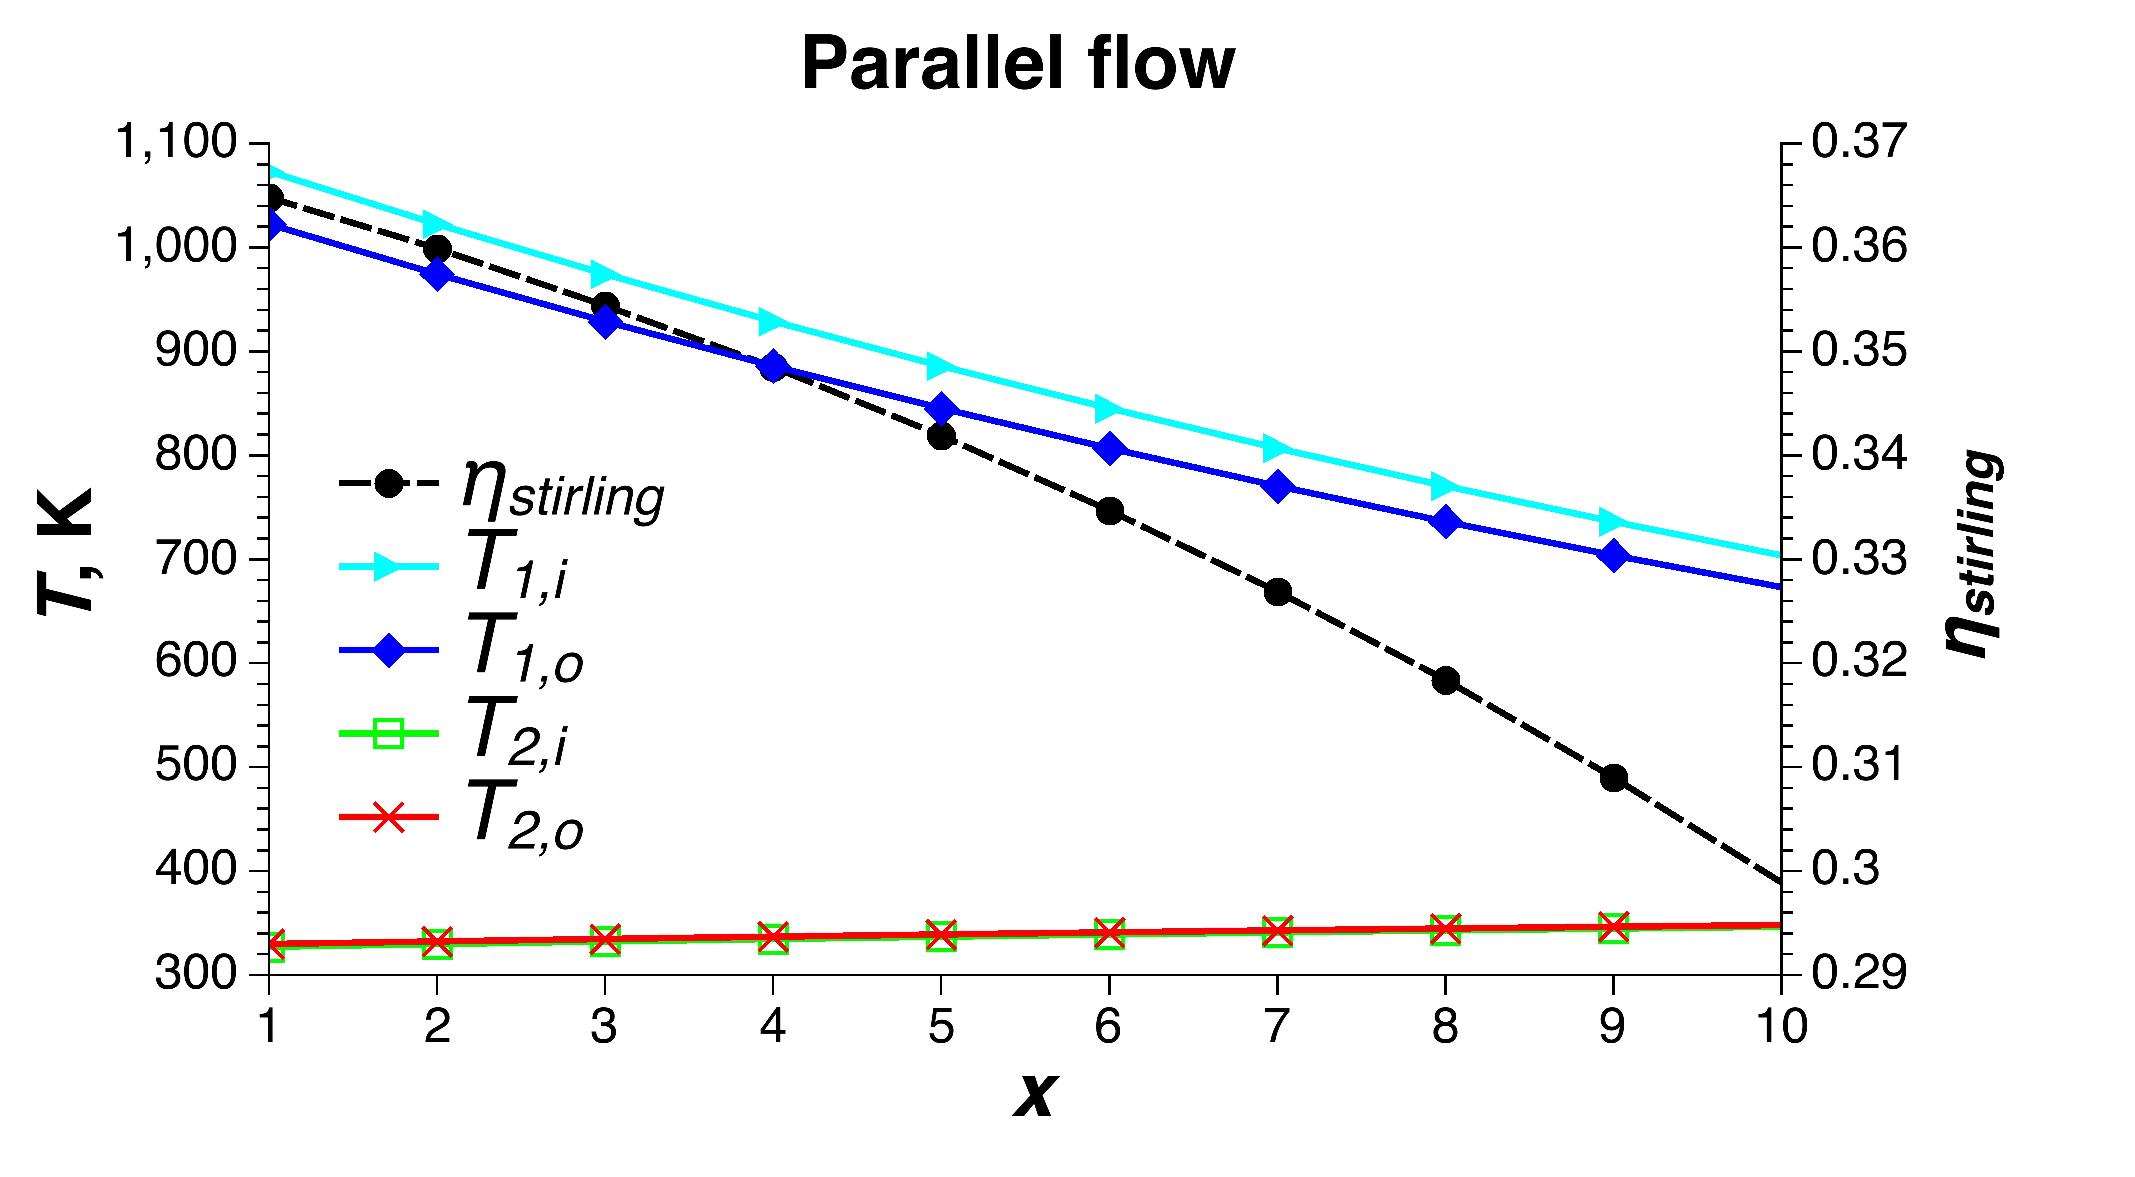
\includegraphics[width = 0.8\columnwidth, angle = 0]{./graphics/Parallelflow}
	\caption{Parallel flow: Temperature series of two fluids and efficiency of Stirling engines in column $x$}
	\label{fig:Parallelflow}
\end{center}
\end{figure}
\noindent \begin{figure}[H]
\begin{center}
	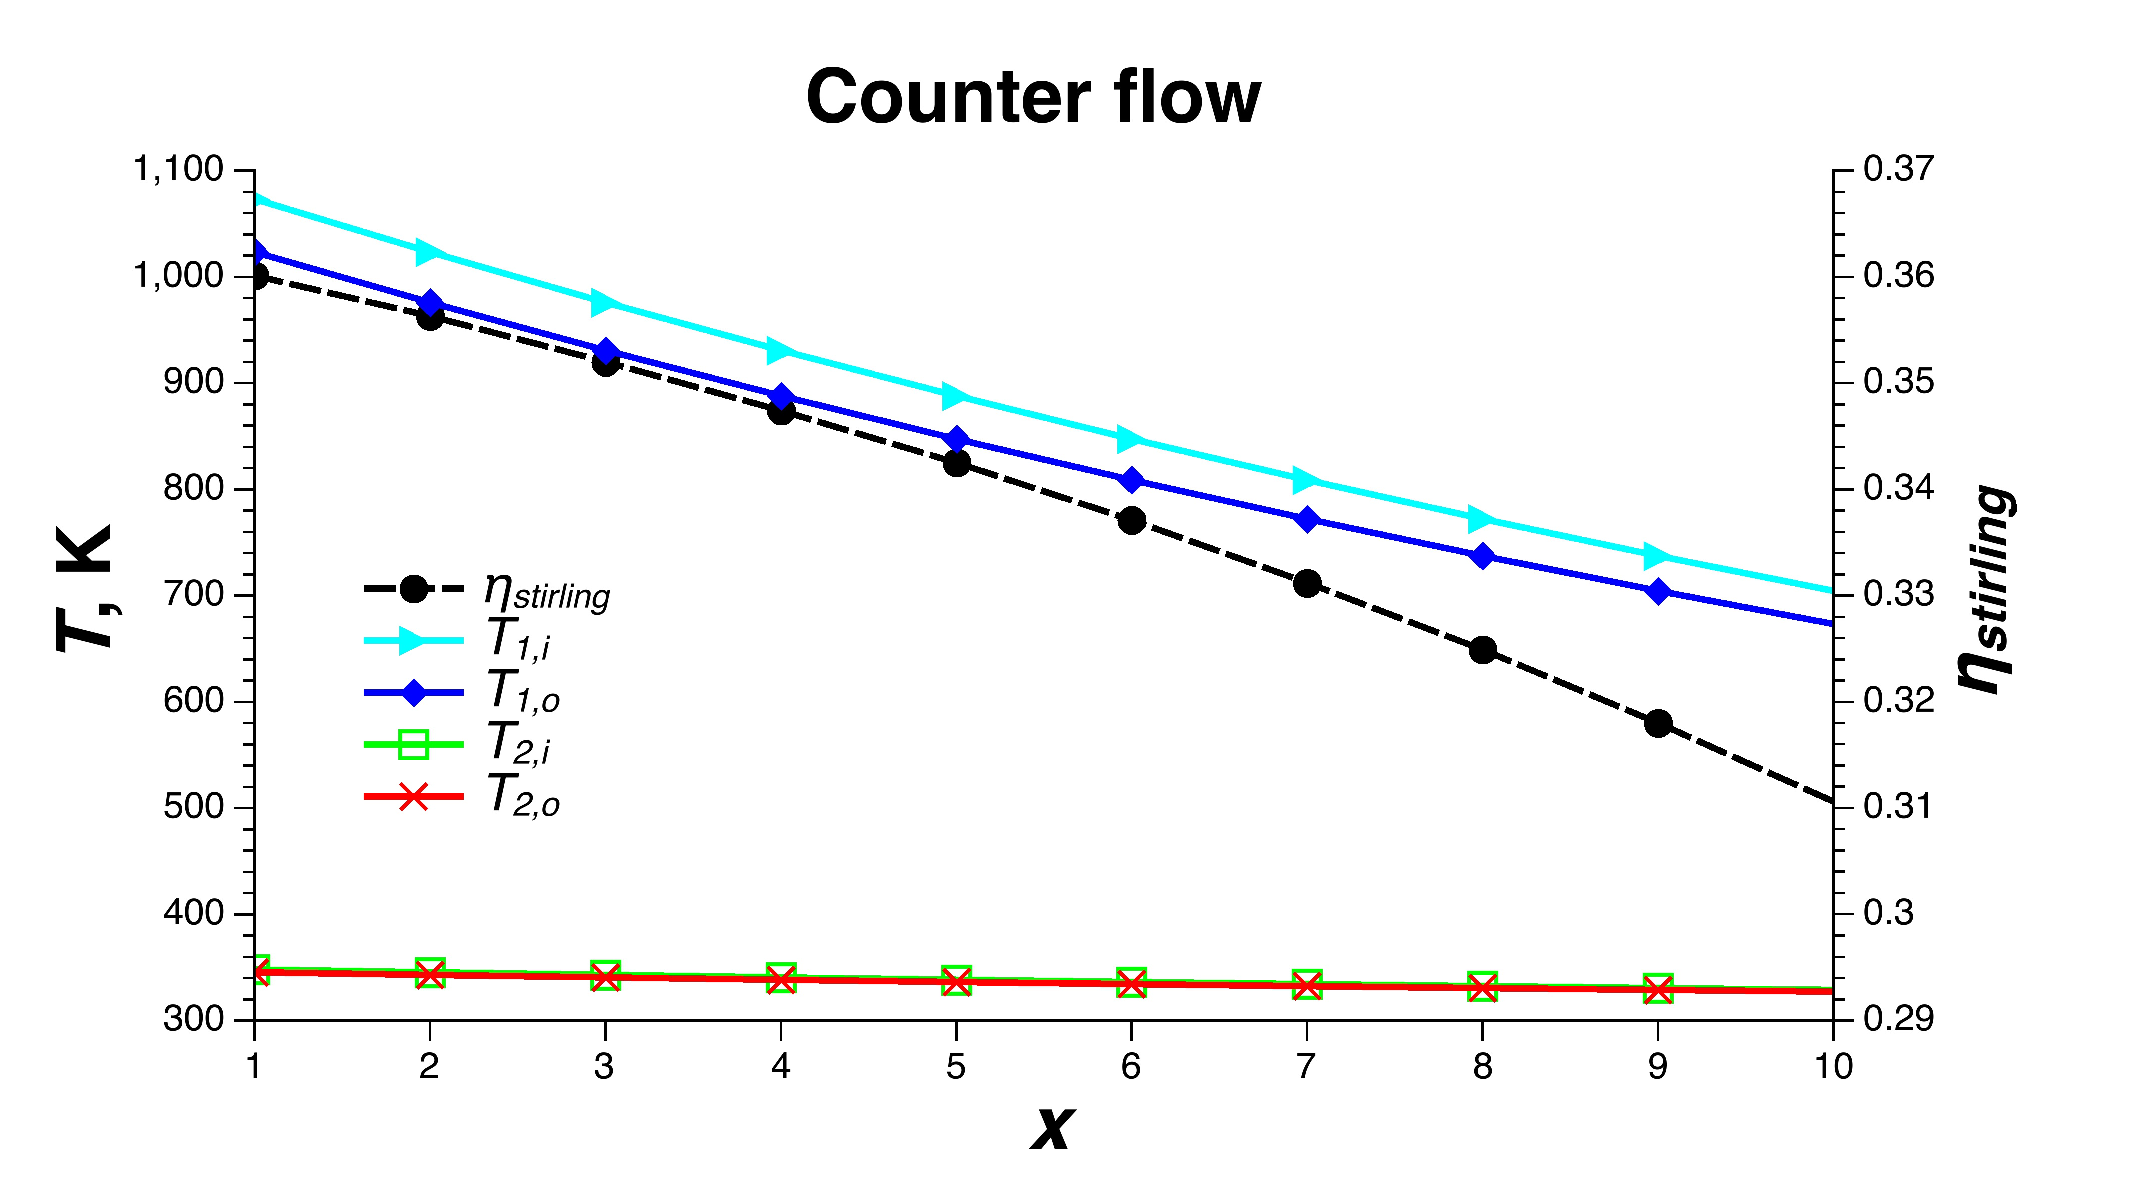
\includegraphics[width = 0.8\columnwidth, angle = 0]{./graphics/Counterflow}
	\caption{Counter flow: Temperature series of two fluids and efficiency of Stirling engines in column $x$}
	\label{fig:Counterflow}
\end{center}
\end{figure}

From Figure~\ref{fig:Parallelflow} and~\ref{fig:Counterflow}, it can be concluded that the temperature increment of cooling fluid is much smaller than the temperature decrement of heating fluid due to their large difference of $c_pq_m$, which leads to a small difference of overall efficiency of Stirling engine array between the two flow types.

To find out a clear difference of the two flow types, a simple model of Stirling engine array was built with air as the heating fluid and water as the cooling fluid. $T_{1,i}, T_{1,o}, T_{2,i}, q_{1,m}$ are fixed and chosen the same values as in the cascade system. Change the value of $q_{2,m}$, and the corresponding Stirling engine array efficiency of the two flow types can be obtained. Figure~\ref{fig:SEAflowtypes} shows the efficiency of Stirling engine array with different $q_{2,m}$ in two flow types. It can be found that counter flow has a higher efficiency than parallel flow, and with lower $q_{2,m}$ comes with higher efficiency difference.

For a system with large difference of $c_pq_m$ of two fluids, that means one fluid can only achieve a small $\Delta T$ compared to the other fluid, will lead to a small difference of two flow types. For a system with similar difference of $c_pq_m$, use the counter flow can achieve a higher efficiency.

\noindent \begin{figure}[H]
\begin{center}
	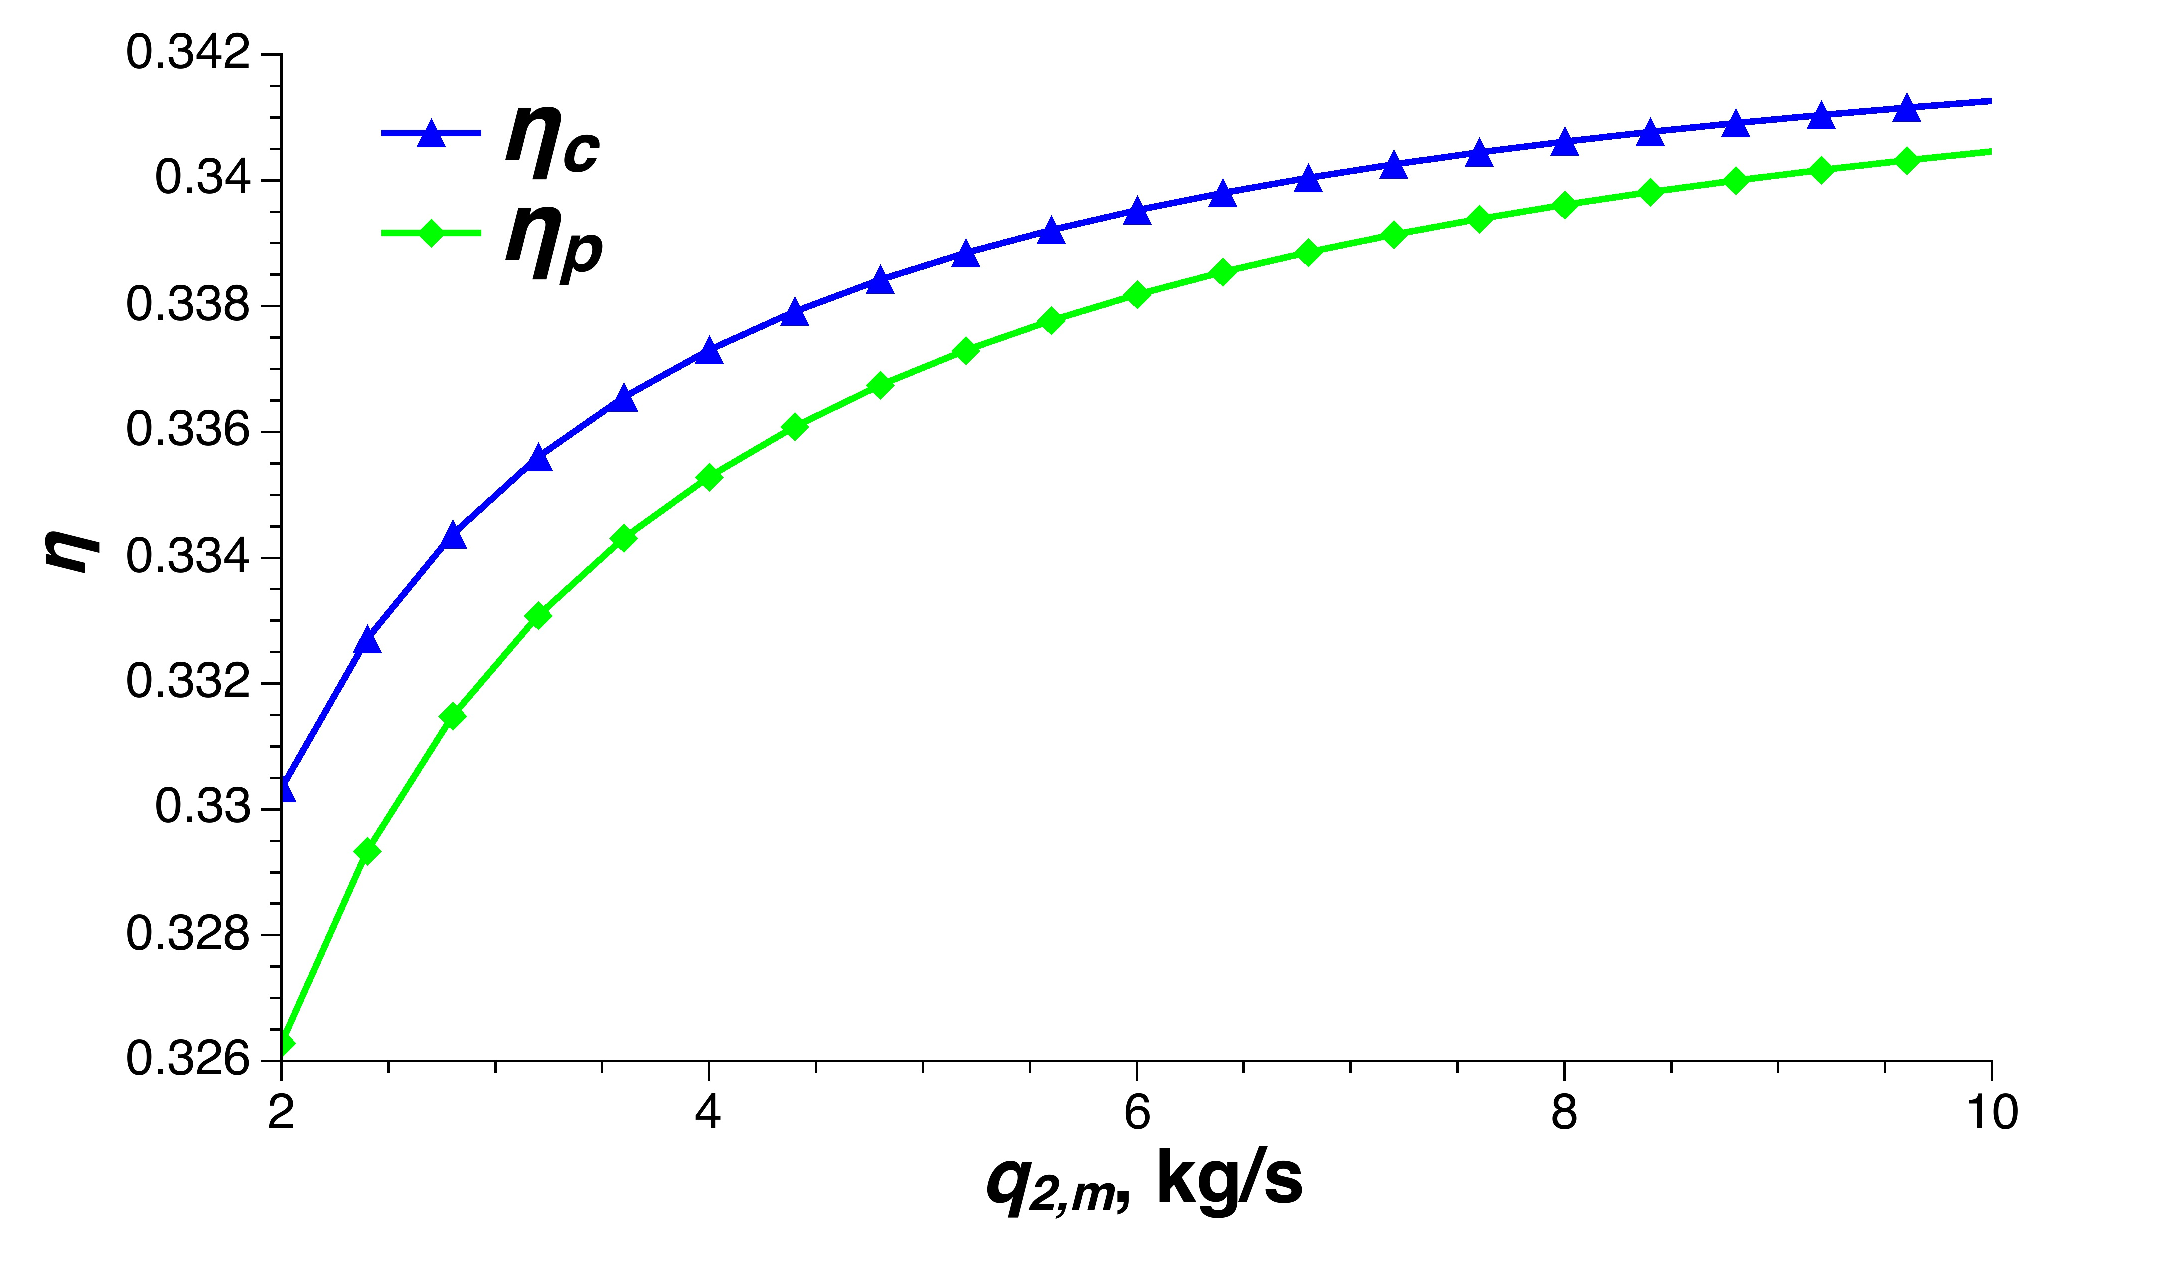
\includegraphics[width = 0.8\columnwidth, angle = 0]{./graphics/SEAflowtypes}
	\caption{Efficiency of Stirling engine array with different $q_{2,m}$}
	\label{fig:SEAflowtypes}
\end{center}
\end{figure}

The first version of cascade system with two different types of collectors and two different power generation methods has been established, including different fluid circuits, with component models. Simulations were carried out and results were compared with corresponding separate systems. Results show that the cascade system can achieve a higher efficiency under certain parameters. The directions to increase the efficiency difference between cascade system and corresponding separate systems were also discussed. higher $I_r$ and $\beta$ is better for a cascade system. The flow type of fluids for heating and cooling Stirling engine array is also required to concern on designing a relative cascade system. Using a cascade system with a different $\beta$ can change the portion of dish collector area of total collector area, which can affect the cost of this technique. The cost analysis and optimization research of the cascade system is not included in this paper, which are worthy for further research later.

\clearpage
\printnomenclature[2.5cm]{}
\clearpage

\bibliography{./bibliography/CascadeSystem}
\bibliographystyle{unsrt}

\clearpage
\appendix

\section{\noindent \label{sec:CTHT}Heat transfer to a constant temperature heat source}

Constant $U$, $T_{c}$, $q_{m}$, $c_{p}$, for a given \nomenclature[S]{$i$}{Inlet}$T_{i}$,

\noindent \begin{center}
\begin{figure}[h]
\begin{centering}
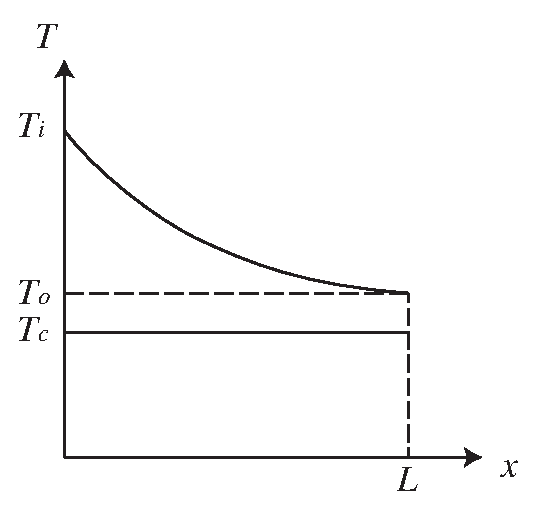
\includegraphics[width=0.6\columnwidth]{graphics/ConstTempHX}
\par\end{centering}

\protect\caption{\label{fig:CTHX}Diagram of heat transfer to a constant temperature heat source}
\end{figure}

\par\end{center}

if $A(x)=Px$, $x$ from $0$ to $L$, $T(x)$ from $T_{i}$ to \nomenclature[S]{$o$}{Outlet}$T_{o}$, 

\begin{equation*}
	q_{m}c_{p}dT(x)=(T_{c}-T(x))UPdx
\end{equation*}

so,

\begin{equation*}
	\frac{dT(x)}{dx}=-\frac{UP}{q_{m}c_{p}}(T(x)-T_{c})
\end{equation*}

Set $F(x)=T(x)-T_{c}$, then $F(0)=T_{i}-T_{c}$, and

\begin{equation*}
	\dfrac{dF(x)}{F(x)}=-\dfrac{UP}{q_{m}c_{p}}dx
\end{equation*}


\begin{equation*}
	F(x)=F(0)\cdot\exp(-\dfrac{UP}{q_{m}c_{p}}x)
\end{equation*}


\begin{equation*}
	\dfrac{F(L)}{F(0)}=\exp(-\dfrac{UPL}{q_{m}c_{p}})
\end{equation*}


That is

\begin{equation*}
	\frac{T_{o}-T_{c}}{T_{i}-T_{c}}=\exp(-\frac{UA}{q_{m}c_{p}})
\end{equation*}
\clearpage{}

\section{\noindent \label{sec:CTCHTHT}Ambient loss of a flow under constant
heat flux}

Constant $U$, $T_{amb}$, $q_{m}$, $c_{p}$, $q^{''}$, for given
$T_{i}$,

\noindent \begin{center}
\begin{figure}[h]
	\noindent \centering{}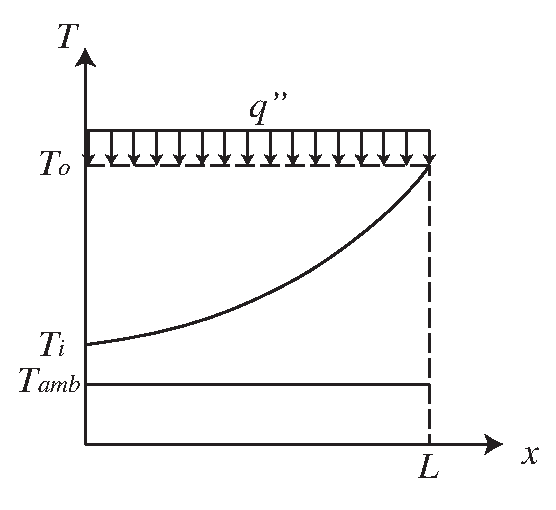
\includegraphics[width=0.8\columnwidth]{graphics/CTCHFHX}
	\protect\caption{\label{fig:CTCHFHX}Diagram of ambient loss of a flow under constant
heat flux}
\end{figure}

\par\end{center}

if $A(x)=Px$, $x$ from $0$ to $L$, $T(x)$ from $T_{i}$ to $T_{o}$,

\begin{equation*}
	q_{m}c_{p}dT(x)=(T_{amb}-T(x))UPdx+q^{''}Pdx
\end{equation*}

so

\begin{equation*}
	\frac{dT(x)}{dx}=-\frac{UP}{q_{m}c_{p}}T(x)+\frac{q^{''}P+UPT_{amb}}{q_{m}c_{p}}
\end{equation*}

Set $G(x)=T(x)-T_{amb}-\dfrac{q^{''}}{U}$, then $G(0)=T_{i}-T_{amb}-\dfrac{q^{''}}{U}$ and

\begin{equation*}
	\dfrac{dG(x)}{G(x)}=-\dfrac{UP}{q_{m}c_{p}}dx
\end{equation*}

\begin{equation*}
	G(x)=G(0)\cdot\exp(-\dfrac{UP}{q_{m}c_{p}}x)
\end{equation*}

\begin{equation*}
	\dfrac{G(L)}{G(0)}=\exp(-\dfrac{UPL}{q_{m}c_{p}})
\end{equation*}

That is

\begin{equation*}
	\frac{T_{o}-T_{amb}-\frac{q^{''}}{U}}{T_{i}-T_{amb}-\frac{q^{''}}{U}}=\exp(-\frac{UA}{q_{m}c_{p}})
\end{equation*}
\clearpage{}

\section{\noindent \label{sec:Stirling-engine-model}Stirling engine model}

A simple Stirling engine model is used for the system. The cycle efficiency is given by \cite{Stine1985}

\begin{equation}
	\eta=\frac{T_{H}-T_{L}}{T_{H}+\text{\ensuremath{\dfrac{1-e}{k-1}}}\cdot\dfrac{T_{H}-T_{L}}{\ln\gamma}}\label{eq:eta_stirling}
\end{equation}


where \nomenclature{$e$}{Regeneration effectiveness of the Stirling engine}$e=\dfrac{T_{R}-T_{L}}{T_{H}-T_{L}}$,\nomenclature{$T_R$}{Regenerator temperature, K}$T_{R}$ is the\emph{ }regenerator temperature, \nomenclature{$c_p$}{Heat capacity of Stirling engine working gas at constant pressure, J/(kg$\cdot$K)}\nomenclature{$c_v$}{Heat capacity of Stirling engine working gas at constant volume, J/(kg$\cdot$K)}$k=\dfrac{c_{p}}{c_{v}}$ for the working gas, $\gamma_{stirling}=\dfrac{V_{max}}{V_{min}}$ is the compression ratio.

The heat transfer diagram is shown in Figure \ref{fig:Heat-transfer-diagram}. Flow 1 is used for heating the hot chamber of Stirling engine, $T_{1i}$ is the inlet temperature, $T_{1o}$ is the outlet temperature. Flow 2 is used for cooling the cold chamber of Stirling engine, $T_{2i}$ is the inlet temperature, $T_{2o}$ is the outlet temperature. \nomenclature{$T_H$}{Highest temperature of expansion space, K}$T_{H}$ is the highest temperature of expansion space, \nomenclature{$T_L$}{Lowest temperature of compression space, K}$T_{L}$ is the lowest temperature of compression space.

\noindent \begin{center}
\begin{figure}[h]
	\noindent \centering{}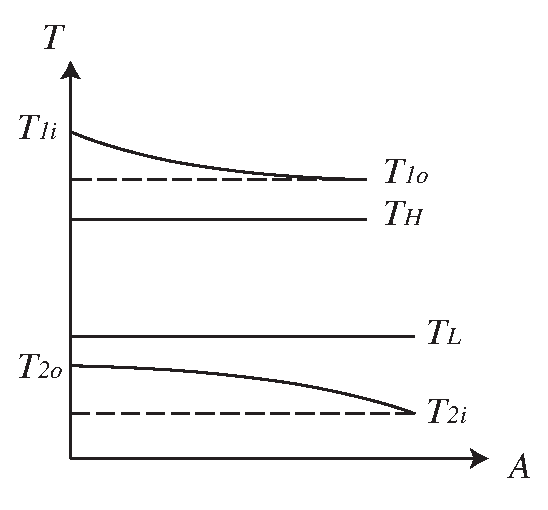
\includegraphics[width=0.6\columnwidth]{graphics/StirilingHT}
	\protect\caption{\label{fig:Heat-transfer-diagram}Heat transfer diagram of Stirling
engine}
\end{figure}

\par\end{center}

According to Appendix \ref{sec:CTHT}, we have

\begin{equation*}
	\dfrac{T_{1o}-T_{H}}{T_{1i}-T_{H}}=\exp(-\dfrac{U_{1}A_{1}}{q_{m,1}c{}_{p1}})
\end{equation*}

and

\begin{equation*}
	\dfrac{T_{2o}-T_{L}}{T_{2i}-T_{L}}=\exp(-\dfrac{U_{2}A_{2}}{q_{m,2}c_{p2}})
\end{equation*}

So known $T_{1o},T_{1i},U_{1},A_{1},q_{m,1},c_{p1},T_{2o},T_{2i},U_{2},A_{2},q_{m,2},c_{p2}$, we can get $T_{H}$ and $T_{L}$, and then use Equation (\ref{eq:eta_stirling}) to get $\eta$.
\nomenclature{$A$}{Area, m$^2$}
\clearpage

\end{document}